% !TEX program = xelatex
% 电子版论文: 无需承诺书与编号页, 摘要页为第一页(符合2026年格式规范第十条), 使用 withoutpreface。
% 纸质版论文: 需承诺书+编号专用页+摘要页, 把下面一行改为:
%   \documentclass[bwprint]{cumcmthesis}
\documentclass[withoutpreface]{cumcmthesis}

% ==================== 封面与编号信息 ====================
\title{快充策略对锂离子电池寿命衰减的影响\\——数据整理、量化建模、寿命预测与策略优化}
\tihao{B}
\baominghao{000000000000}
\schoolname{XX大学}
\membera{姓名A}
\memberb{姓名B}
\memberc{姓名C}
\supervisor{指导教师}
\yearinput{2026}
\monthinput{08}
\dayinput{01}

% 代码清单中的中文注释字体设置（与正文字体一致，防止中文显示为方块）
\lstset{basicstyle=\small\ttfamily\song}
% 等宽字体回退: 支持 ≈ ∈ 等符号 (Windows 上若无 DejaVu 则沿用默认)
\IfFontExistsTF{DejaVu Sans Mono}{\setmonofont{DejaVu Sans Mono}}{}

\begin{document}

% 电子版提交时不要承诺书与编号页(withoutpreface 已跳过)，\maketitle 生成标题
\maketitle

\begin{abstract}
本文基于 MIT--Stanford 公开锂离子电池循环老化数据集，围绕“快充策略--充电时间--寿命衰减”的定量关系，依次完成数据整理、量化建模、寿命预测与策略优化四项递进任务。

对于问题一，系统整理了 124 个 A123 18650 磷酸铁锂电池的充电策略参数（第一阶段倍率 $C_1$、切换 SOC $Q_1$、第二阶段倍率 $C_2$）、循环寿命、SOH 衰减曲线与充电时间，完成异常循环清洗、格式归一化与协议类型区分；寿命分布跨度约 15 倍（148--2235），并识别出典型长寿命策略（中高 SOC 区间倍率温和，$C_2\le 4.4$C）与短寿命策略（$C_2\ge 5.5$C）。

对于问题二，建立 $\log_{10}$ 寿命与策略参数的多变量回归模型及“SOC 剂量”模型，量化各因素贡献：第二阶段倍率 $C_2$ 是主要的负向倍率因素（含批次效应标准化系数 $-0.040$，偏相关 $-0.250$），充电时间与寿命正相关（偏相关 $+0.363$）；单位高倍率电量在中高 SOC 区间的寿命损伤比低 SOC 区间高约 16\%（$m_2$ 系数 $-0.424$ vs $m_1$ $-0.367$），验证了不同 SOC 区间高倍率影响的显著差异。

对于问题三，从早期循环提取 SOH 衰减率、波动、充电时间漂移等特征，建立梯度提升寿命预测模型，5 折$\times$8 次重复交叉验证下以前 20 个循环预测寿命的 MAPE 达 15.3\%（$R^2=0.77$）；特征重要性分析表明充电时间波动与 SOH 残差波动为主导特征，近中期 SOH 预测误差小于 1.2\%。

对于问题四，构建校准的充电时间模型与剂量型寿命响应面，在实验覆盖的合理邻域内做多目标网格寻优得到 Pareto 前沿，膝点对应策略为 3.6C(80\%)-3.6C（充电时间 13.3 min、预测寿命 1794、数据实测 2081），更快备选为 4C(80\%)-4C（12.5 min、实测 1570），两者均为数据已验证的优解，同时给出了外推风险边界。

\keywords{锂离子电池\quad 快速充电\quad 循环寿命\quad SOC 区间\quad 剂量模型\quad 寿命预测\quad Pareto 优化}
\end{abstract}

% ==================== 一、问题重述 ====================
\section{问题重述}

锂离子电池在循环使用过程中可用容量逐渐下降，通常以健康状态 $\mathrm{SOH}=Q_{\mathrm{current}}/Q_{\mathrm{initial}}\times100\%$ 表征老化程度，当 SOH 降至 80\% 时认为达到寿命终止条件。快充能显著缩短补能时间，但较高充电电流会加剧极化、热效应与副反应，加快容量衰减。不同 SOC 区间内电池对充电电流的敏感程度不同：低 SOC 区间采用较大电流有助于缩短充电时间，而中高 SOC 区间继续高倍率充电则可能加剧老化。

本数据集为 MIT--Stanford 公开锂离子电池循环老化数据集\upcite{ref1}，共 124 个 A123 18650 磷酸铁锂电池（额定容量 1.1 Ah），分三个批次（41/43/40）。充电采用分段快充策略，可表示为：先以 $C_1$ 倍率从 0\% SOC 充电至 $Q_1$，再以 $C_2$ 倍率从 $Q_1$ 充电至 80\% SOC，最后以 1C 恒流--恒压（CC-CV）模式充电至满电。不同电池的差异主要体现于 $C_1$、$Q_1$、$C_2$ 三个参数。需要说明的是，本文中 "C" 表示充放电倍率（即以额定容量为基准的电流倍数，如 3.6C 表示充电电流为 3.6$\times$1.1 A），并非电荷量的库仑单位。

需要解决以下四个问题：
\begin{enumerate}
\item 对原始循环实验数据进行整理，提取各电池的充电策略、充电时间、SOH 变化及循环寿命等关键信息；给出典型长寿命策略和短寿命策略，并从充电倍率、SOC 区间和充电时间角度进行初步解释。
\item 建立充电策略参数与电池寿命衰减之间的定量关系模型，重点分析不同 SOC 区间内充电电流倍率对寿命的影响，量化 $C_1$、$Q_1$、$C_2$ 及充电时间的贡献，并给出各因素及交互作用的影响程度排序。
\item 基于给定快充策略下电池早期循环数据，建立寿命预测模型，预测电池未来 SOH 衰减趋势或达到寿命终止条件时的循环次数，并讨论早期循环长度与策略参数的作用。
\item 设计兼顾充电时间与寿命衰减的快充策略优化方法，给出推荐策略，并与典型长寿命、短寿命策略对比，说明其合理性、适用范围和可能的外推风险。
\end{enumerate}

% ==================== 二、问题分析 ====================
\section{问题分析}

问题一的核心是数据整理与规律初探：需先解析三段式快充策略参数、校准充电时间单位、清洗异常循环，再对寿命分布做分批次统计，并从多参数角度解释长短寿命差异。

问题二的核心是因果量化：寿命跨度达约 15 倍，需用回归模型解耦 $C_1$、$Q_1$、$C_2$、充电时间的贡献。考虑到实验设计存在混杂与批次效应，采用含批次虚拟变量的多变量回归，并构造“SOC 剂量”变量 $m_1=C_1Q_1/100$、$m_2=C_2(80-Q_1)/100$ 直接检验不同 SOC 区间高倍率影响的差异。

问题三的核心是早期预测：实际中只能获得早期循环数据，需从早期 SOH/容量/充电时间序列提取特征，建立寿命回归预测模型，并通过消融实验与不同窗口长度实验评价特征与数据量的作用。

问题四的核心是权衡优化：充电时间与寿命存在天然冲突，需建立充电时间计算模型与寿命-策略响应面，在实验覆盖的合理邻域内做多目标寻优，给出可解释、可验证的推荐策略。

四个问题逐层递进，形成“整理 $\rightarrow$ 量化 $\rightarrow$ 预测 $\rightarrow$ 优化”的完整链条，前一问题的输出作为后一问题的输入。整体研究流程见图 \ref{fig:fig20}。

\begin{figure}[htbp]
\centering
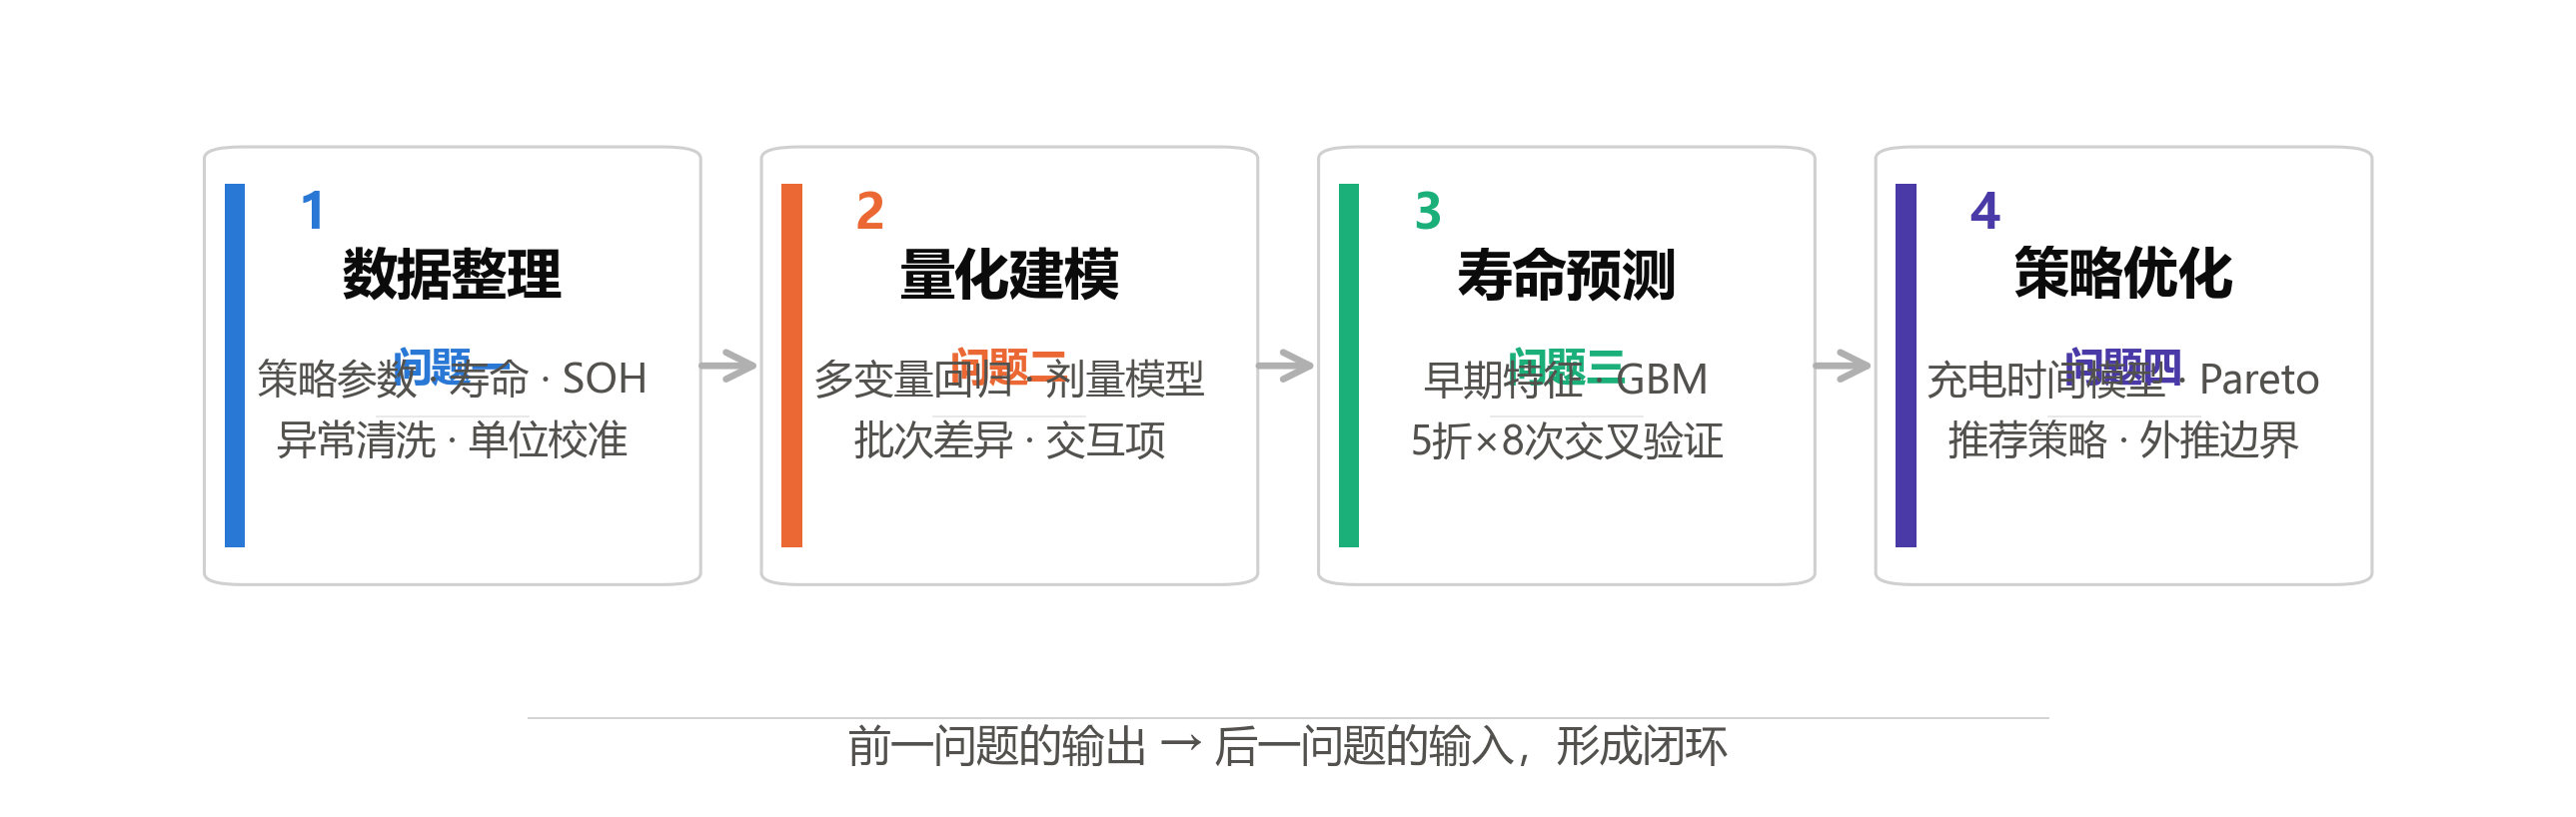
\includegraphics[width=0.92\textwidth]{figures/fig20.png}
\caption{本文研究流程（四问题递进）}
\label{fig:fig20}
\end{figure}

% ==================== 三、模型假设 ====================
\section{模型假设}

基于对数据集结构与电池老化机理的分析，提出如下假设：

\begin{enumerate}
\item 各电池初始状态一致，SOH 以首循环放电容量为基准归一化；80\% SOH 为寿命终止（EOL）阈值。该假设保证了同一策略下多个电池的寿命标签可比。
\item 充电时间定义为快充段（0$\sim$80\% SOC）耗时，不含 80\%$\sim$100\% 的 CC-CV 补电阶段。数据验证显示各电池的 CC-CV 补电阶段电流均按 C/50 截止，时长由电流决定、与快充段解耦，故单独度量快充段更利于策略比较。
\item 批次内环境（温度、夹具、工艺）条件一致；批次间差异通过批次效应项吸收，不假定批次间可互换。该假设将难以观测的批次差异显式建模，避免其与策略效应混淆。
\item 不同 SOC 区间的高倍率充电对老化的贡献具有可加性（剂量叠加假设），且效应在观测参数范围内近似线性。该假设是剂量模型（第 7.3 节）的基础，残差诊断（第 7.7 节）验证了其近似合理性。
\item 优化仅在实验覆盖的参数水平及其合理邻域内进行，不向未经验证的高倍率或 SOC 区间外推。该假设确保优化结果的可验证性与工程安全性。
\end{enumerate}

上述假设在相应章节中均通过数据或残差诊断进行了检验，若有违背之处已在模型的适用范围与不足中予以说明。

% ==================== 四、符号说明 ====================
\section{符号说明}

\begin{table}[H]
\centering
\caption{主要符号说明}
\label{tab:symbol}
\begin{tabular}{cll}
\toprule
符号 & 含义 & 单位 \\
\midrule
$C_1$ & 第一阶段充电倍率 & C \\
$Q_1$ & 第一阶段结束（切换）时的 SOC & \% \\
$C_2$ & 第二阶段充电倍率 & C \\
$T_{80}$ & 快充段（0$\sim$80\% SOC）充电时间 & min \\
$\mathrm{SOH}$ & 健康状态（容量保持率） & \% \\
$L$ & 循环寿命（cycle\_life） & 循环 \\
$m_1$ & 低 SOC 区间高倍率电量剂量 $=C_1Q_1/100$ & Ah \\
$m_2$ & 中高 SOC 区间高倍率电量剂量 $=C_2(80-Q_1)/100$ & Ah \\
$k$ & 早期循环窗口长度 & 循环 \\
MAPE & 平均绝对百分比误差 & \% \\
$R^2$ & 决定系数 & 无量纲 \\
\bottomrule
\end{tabular}
\end{table}

% ==================== 五、数据整理与预处理 ====================
\section{数据整理与预处理}

\subsection{数据来源与结构}

原始数据为三个 MATLAB v7.3（HDF5）文件，对应三个实验批次，见表 \ref{tab:data}。每个电池包含策略字符串（policy\_readable）、循环寿命标签（cycle\_life）、逐循环汇总（放电容量、内阻、温度、充电时间）与逐循环电流/电压时序。

关于数据口径需作三点说明：（1）\textbf{循环寿命定义}：cycle\_life 为电池放电容量首次衰减至 0.88 Ah（额定容量 1.1 Ah 的 80\%）时的循环数；对实验期间未衰减至该阈值的电池，取最后一个测试循环作为寿命标签。（2）\textbf{电池数量}：原始文件共含 140 条电池记录；为与题目所述的 124 个电池口径一致，合并了 5 个同一物理电池的延续测试段（批次 2 中有 5 个电池为批次 1 电池的延续），并剔除 12 个未完成循环或存在数据采集异常的电池，最终得到 124 个有效电池（批次 1/2/3 分别为 41/43/40 个），均具有有效 cycle\_life 标签。（3）\textbf{批次 3 协议}：批次 3 的第二个倍率为放电倍率（newstructure），充电为"$C_1$ 充至 $Q_1$ 后接 1C CC-CV"，见后文。

\begin{table}[htbp]
\centering
\caption{数据集构成}
\label{tab:data}
\begin{tabular}{cccc}
\toprule
批次 & 电池数 & 充电策略范围 & 协议类型 \\
\midrule
data\_1（2017-05） & 41 & 3.6C$\sim$8C & 标准 \\
data\_2（2018-04） & 43 & 1C$\sim$6C（激进攻略居多） & 标准 \\
data\_3（2018-08） & 40 & 3.7C$\sim$5.9C & newstructure \\
\bottomrule
\end{tabular}
\end{table}

\subsection{关键提取与清洗}

\textbf{（1）策略参数解析。}从策略字符串 \texttt{C1C(Q1\%)-C2C} 正则提取 $C_1$、$Q_1$、$C_2$，处理了两类格式异常：截断型（如 \texttt{80\%)-3.6C}，参考电池）依据充电时间反推 $C_1=C_2$；缺单位型（如 \texttt{4C(31\%)-5}）容错解析。

\textbf{（2）协议类型区分。}经核对批次 3 电流曲线，其策略字符串中的第二个倍率实际为放电倍率，充电阶段为“$C_1$ 充至 $Q_1$，后接 1C CC-CV”，与批次 1、2 不同，故单独标记为 newstructure 协议。

\textbf{（3）异常循环清洗。}个别循环放电容量相对前值突变超过 20\%（如 data\_1\_cell0 循环 11 出现 SOH$\approx$143\% 的跳变），判定为测量异常并剔除。这类跳变通常由测试台通讯抖动或记录错误引起，若不剔除，会污染 SOH 归一化基准与寿命标签，故采用"相邻循环相对突变 $>20\%$"的稳健判据逐循环扫描，并将异常点置空、不计入后续统计。

\textbf{（4）数据质量筛选。}结合第 2.1 节的口径处理，剔除未完成循环（如 data\_3\_cell23、data\_3\_cell32 的 cycle\_life 缺失）及测试后期容量未降至 0.88 Ah 阈值、数据采集异常的电池，最终保留 124 个有效电池。

\textbf{（5）充电时间单位校准。}依据“充电至 80\% SOC 的理论时间”验证，确认单位均为分钟（如 3.6C(80\%) 理论 $0.8/3.6\times60=13.33$ min，实测 13.34 min），并确认充电时间对应快充段（0$\sim$80\% SOC）耗时。

整理后的电池级汇总表节选见表 \ref{tab:battery}。

\begin{table}[htbp]
\centering
\caption{电池级汇总表（节选）}
\label{tab:battery}
\begin{tabular}{cccccccc}
\toprule
电池 & 批次 & 策略 & $C_1$(C) & $Q_1$(\%) & $C_2$(C) & 循环寿命 & 充电时间(min) \\
\midrule
data\_1\_cell00 & data\_1 & 3.6C(80\%)-3.6C & 3.6 & 80 & 3.6 & 1850 & 13.5 \\
data\_1\_cell03 & data\_1 & 4C(80\%)-4C & 4.0 & 80 & 4.0 & 1432 & 12.4 \\
data\_2\_cell00 & data\_2 & 1C(4\%)-6C & 1.0 & 4 & 6.0 & 300 & 12.8 \\
data\_2\_cell01 & data\_2 & 2C(10\%)-6C & 2.0 & 10 & 6.0 & 148 & 12.5 \\
\bottomrule
\end{tabular}
\end{table}

% ==================== 六、问题一 ====================
\section{问题一：寿命分布统计与典型策略分析}

\subsection{寿命分布统计}

全部 124 个有效电池的循环寿命分布见表 \ref{tab:life-dist}，分布直方图见图 \ref{fig:fig1}。寿命跨度约 15 倍（最小值 148、最大值 2235），说明充电策略对寿命具有极显著影响。从分布形态看，寿命整体呈右偏（长尾位于 1000$\sim$2235），中位数 736 显著低于均值水平，反映存在一批寿命特别短（$<300$）的激进策略电池拉低了整体；同时分布并非单峰，而是由三个批次混合而成，各批次寿命重心明显不同。这种"批次混合 + 策略驱动"的分布特征，决定了后续分析必须同时考虑策略参数与批次效应。

\begin{table}[htbp]
\centering
\caption{寿命总体分布}
\label{tab:life-dist}
\begin{tabular}{ccccccc}
\toprule
统计量 & 最小值 & 25\%分位 & 中位数 & 75\%分位 & 最大值 & 样本数 \\
\midrule
值 & 148 & 499 & 736 & 946 & 2235 & 124 \\
\bottomrule
\end{tabular}
\end{table}

\begin{figure}[htbp]
\centering
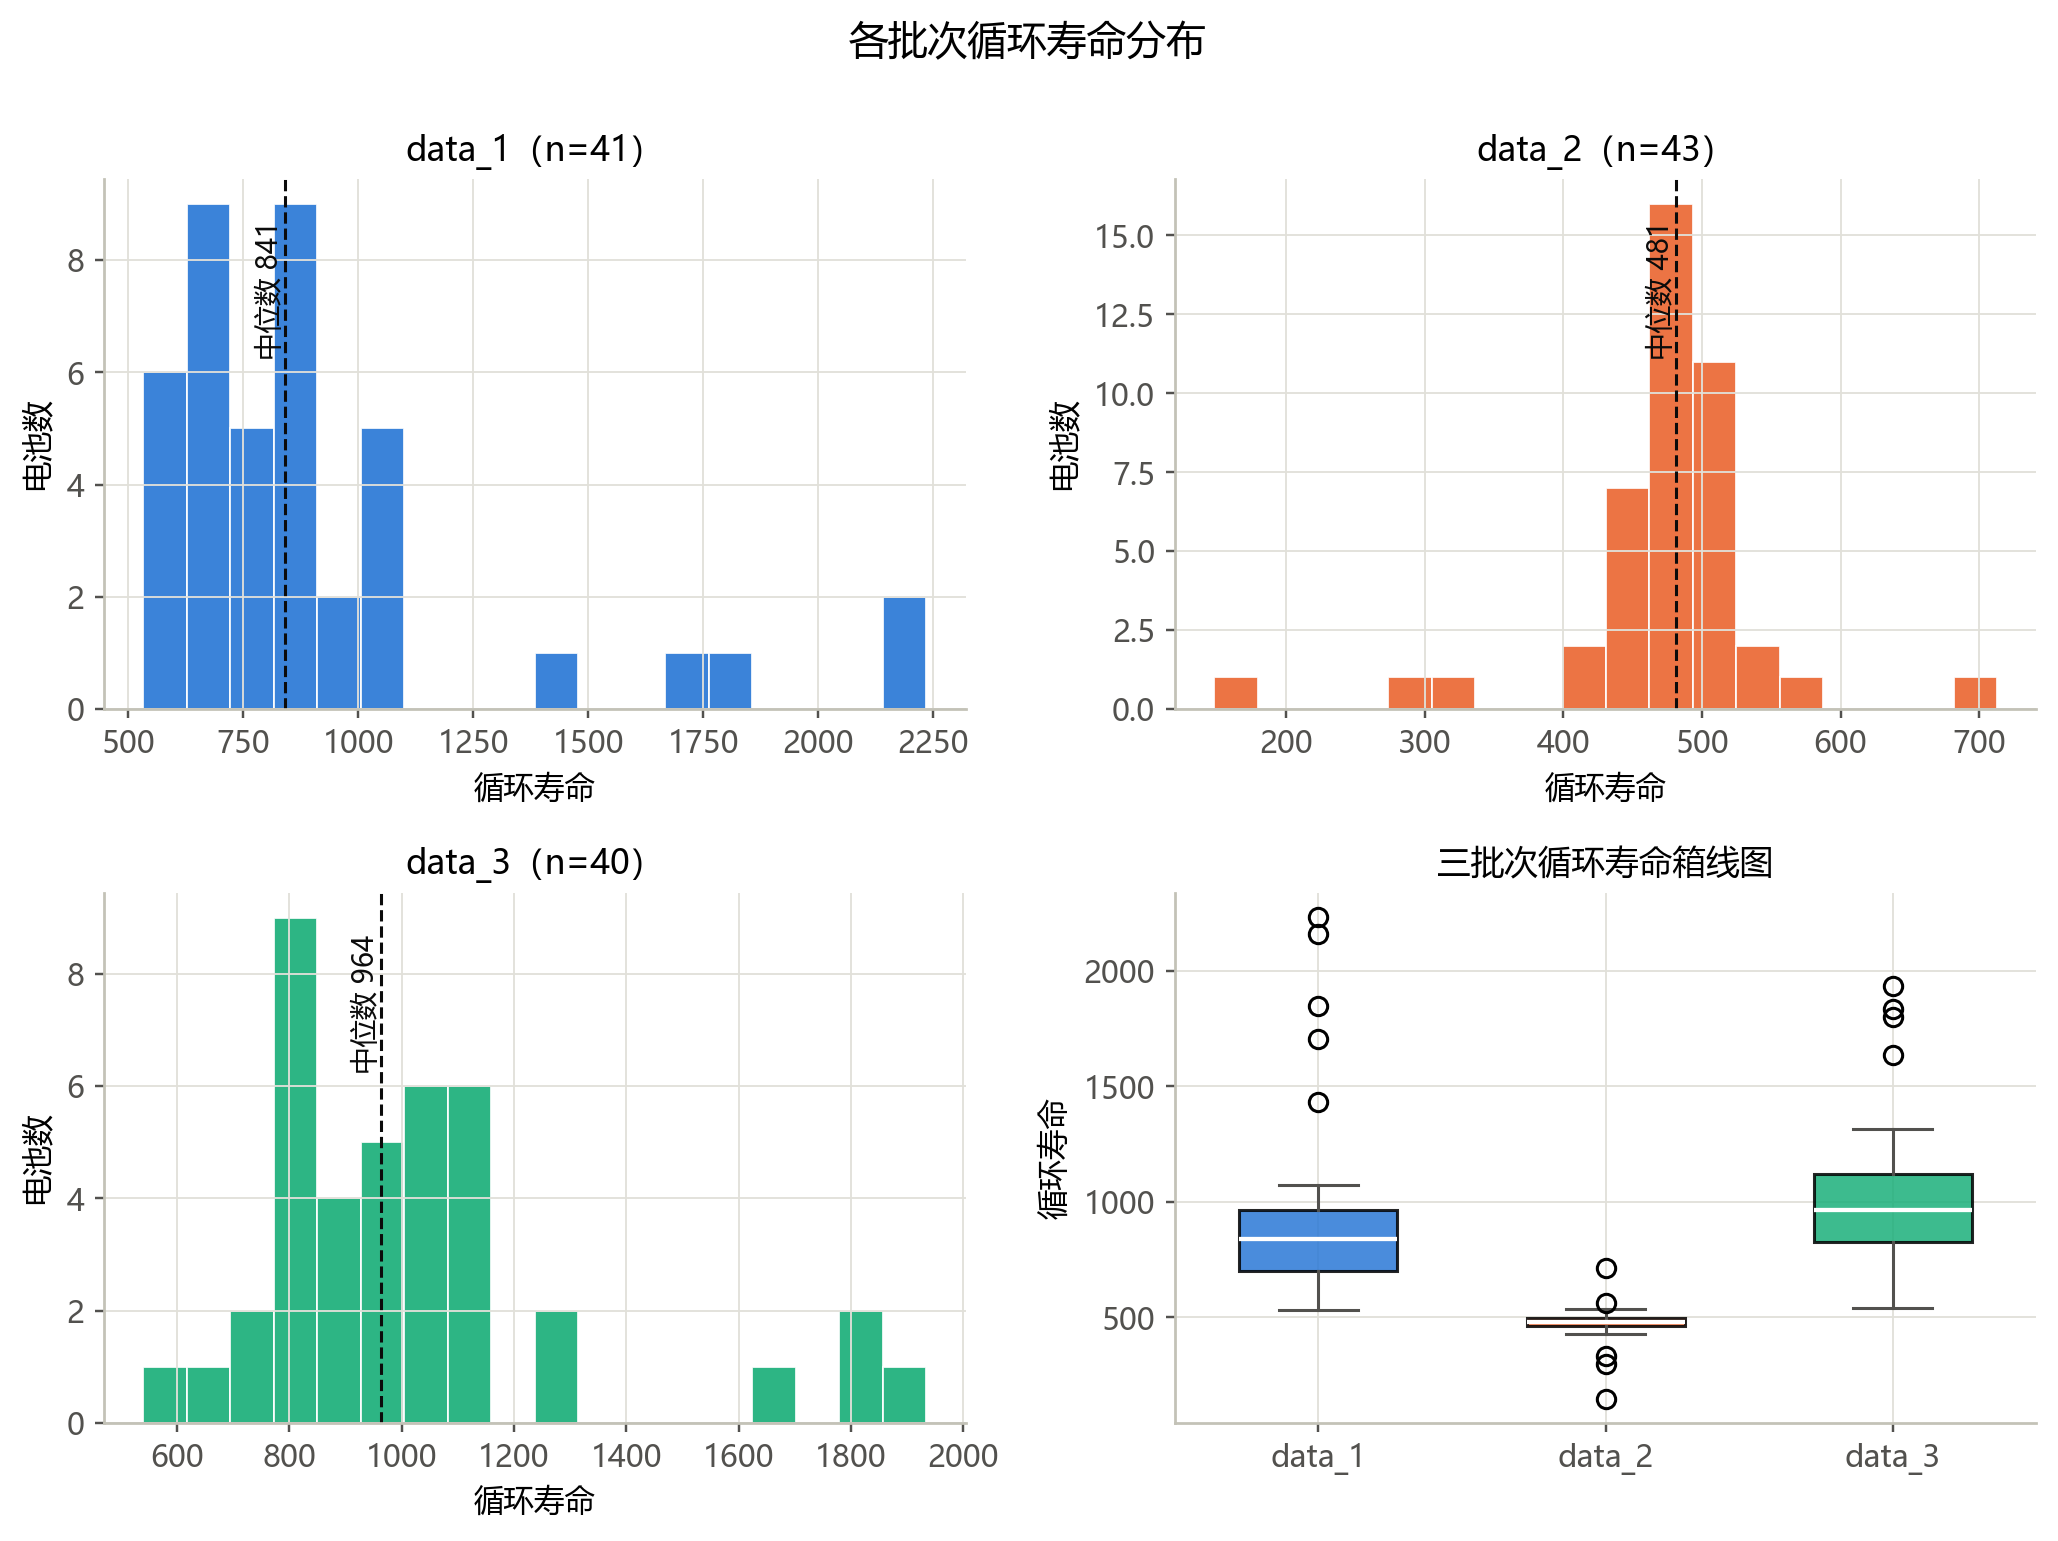
\includegraphics[width=0.95\textwidth]{figures/fig1.png}
\caption{各批次循环寿命分布直方图}
\label{fig:fig1}
\end{figure}

三个批次寿命分布差异显著（表 \ref{tab:batch-dist}）：批次 2 整体寿命最短（中位数 480），因其实验设计集中于高倍率激进攻略（$C_2$ 多在 4$\sim$6C）；批次 3（newstructure）整体寿命最长（中位数 962）。由于三个批次策略参数空间与环境条件不完全一致，后续策略间比较优先在同一批次内进行。

\begin{table}[htbp]
\centering
\caption{各批次寿命分布}
\label{tab:batch-dist}
\begin{tabular}{cccccc}
\toprule
批次 & n & min & 中位数 & max & 均值 \\
\midrule
data\_1 & 41 & 533 & 841 & 2235 & 920 \\
data\_2 & 43 & 148 & 481 & 713 & 473 \\
data\_3 & 40 & 540 & 964 & 1934 & 1031 \\
\bottomrule
\end{tabular}
\end{table}

\subsection{典型长寿命与短寿命策略识别}

对 standard 协议（批次 1+2）各策略的寿命进行统计，按平均寿命排序，选取典型长寿命（前 5）与短寿命（后 5）策略，结果见表 \ref{tab:long}、表 \ref{tab:short}，其 SOH 衰减曲线见图 \ref{fig:fig3}。

\begin{table}[htbp]
\centering
\caption{典型长寿命策略}
\label{tab:long}
\begin{tabular}{ccccccc}
\toprule
策略 & 电池数 & 平均寿命 & $C_1$(C) & $Q_1$(\%) & $C_2$(C) & 充电时间(min) \\
\midrule
3.6C(80\%)-3.6C & 3 & 2081 & 3.6 & 80 & 3.6 & 13.6 \\
4C(80\%)-4C & 2 & 1570 & 4.0 & 80 & 4.0 & 12.3 \\
4.4C(80\%)-4.4C & 1 & 1073 & 4.4 & 80 & 4.4 & 11.6 \\
5.4C(40\%)-3.6C & 1 & 1053 & 5.4 & 40 & 3.6 & 11.4 \\
6C(30\%)-3.6C & 1 & 1013 & 6.0 & 30 & 3.6 & 11.7 \\
\bottomrule
\end{tabular}
\end{table}

\begin{table}[htbp]
\centering
\caption{典型短寿命策略}
\label{tab:short}
\begin{tabular}{ccccccc}
\toprule
策略 & 电池数 & 平均寿命 & $C_1$(C) & $Q_1$(\%) & $C_2$(C) & 充电时间(min) \\
\midrule
2C(10\%)-6C & 1 & 148 & 2.0 & 10 & 6.0 & 12.5 \\
1C(4\%)-6C & 1 & 300 & 1.0 & 4 & 6.0 & 12.8 \\
2C(7\%)-5.5C & 1 & 335 & 2.0 & 7 & 5.5 & 12.2 \\
5.6C(65\%)-3C & 1 & 429 & 5.6 & 65 & 3.0 & 12.1 \\
6C(52\%)-3.5C & 1 & 429 & 6.0 & 52 & 3.5 & 11.0 \\
\bottomrule
\end{tabular}
\end{table}

\begin{figure}[htbp]
\centering
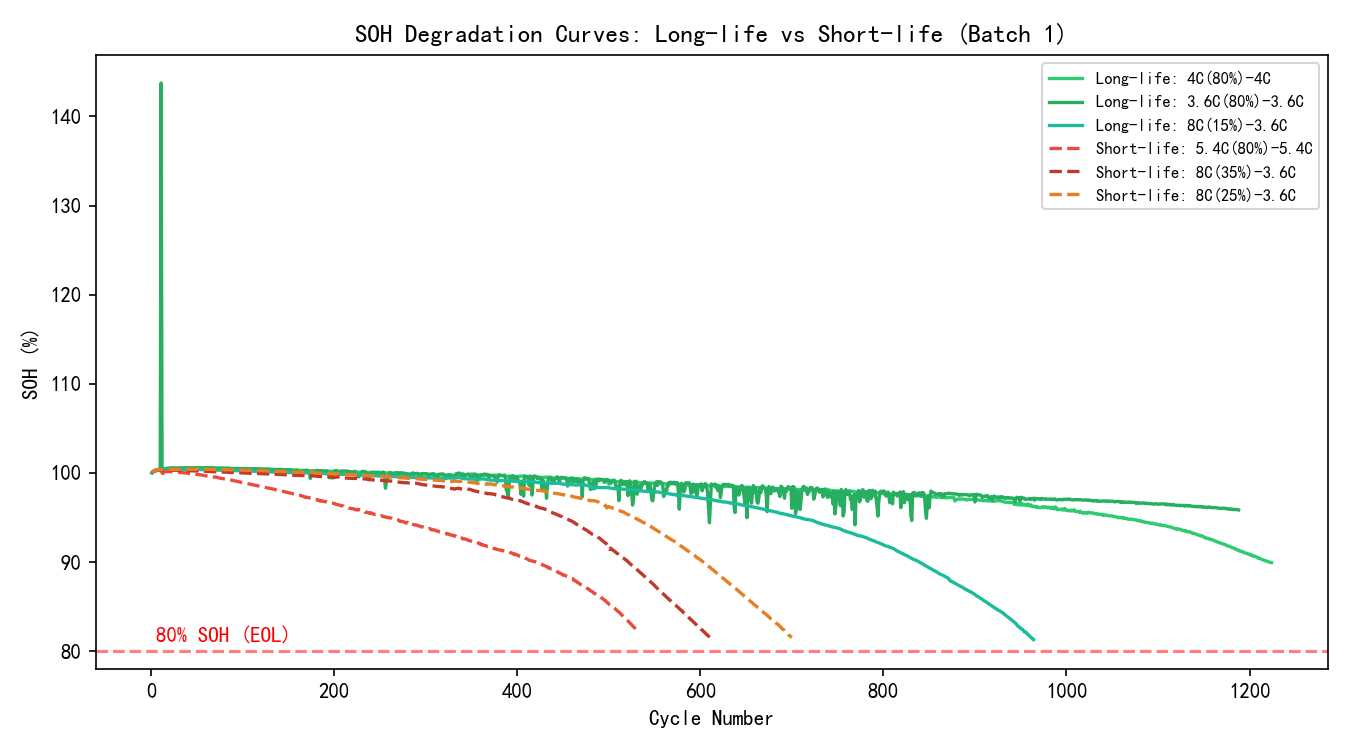
\includegraphics[width=0.8\textwidth]{figures/fig3.png}
\caption{典型长/短寿命电池 SOH 衰减曲线（批次 1）}
\label{fig:fig3}
\end{figure}

\subsection{差异机理解释}

对 standard 协议 84 个电池计算循环寿命与各参数的 Pearson 相关系数（表 \ref{tab:corr}，偏回归关系见图 \ref{fig:fig2} 与图 \ref{fig:fig4}）。

\begin{table}[htbp]
\centering
\caption{cycle\_life 与各参数相关系数}
\label{tab:corr}
\begin{tabular}{ccccc}
\toprule
参数 & $C_1$ & $Q_1$ & $C_2$ & 充电时间(min) \\
\midrule
相关系数 $r$ & 0.026 & 0.423 & -0.418 & 0.330 \\
\bottomrule
\end{tabular}
\end{table}

\begin{figure}[htbp]
\centering
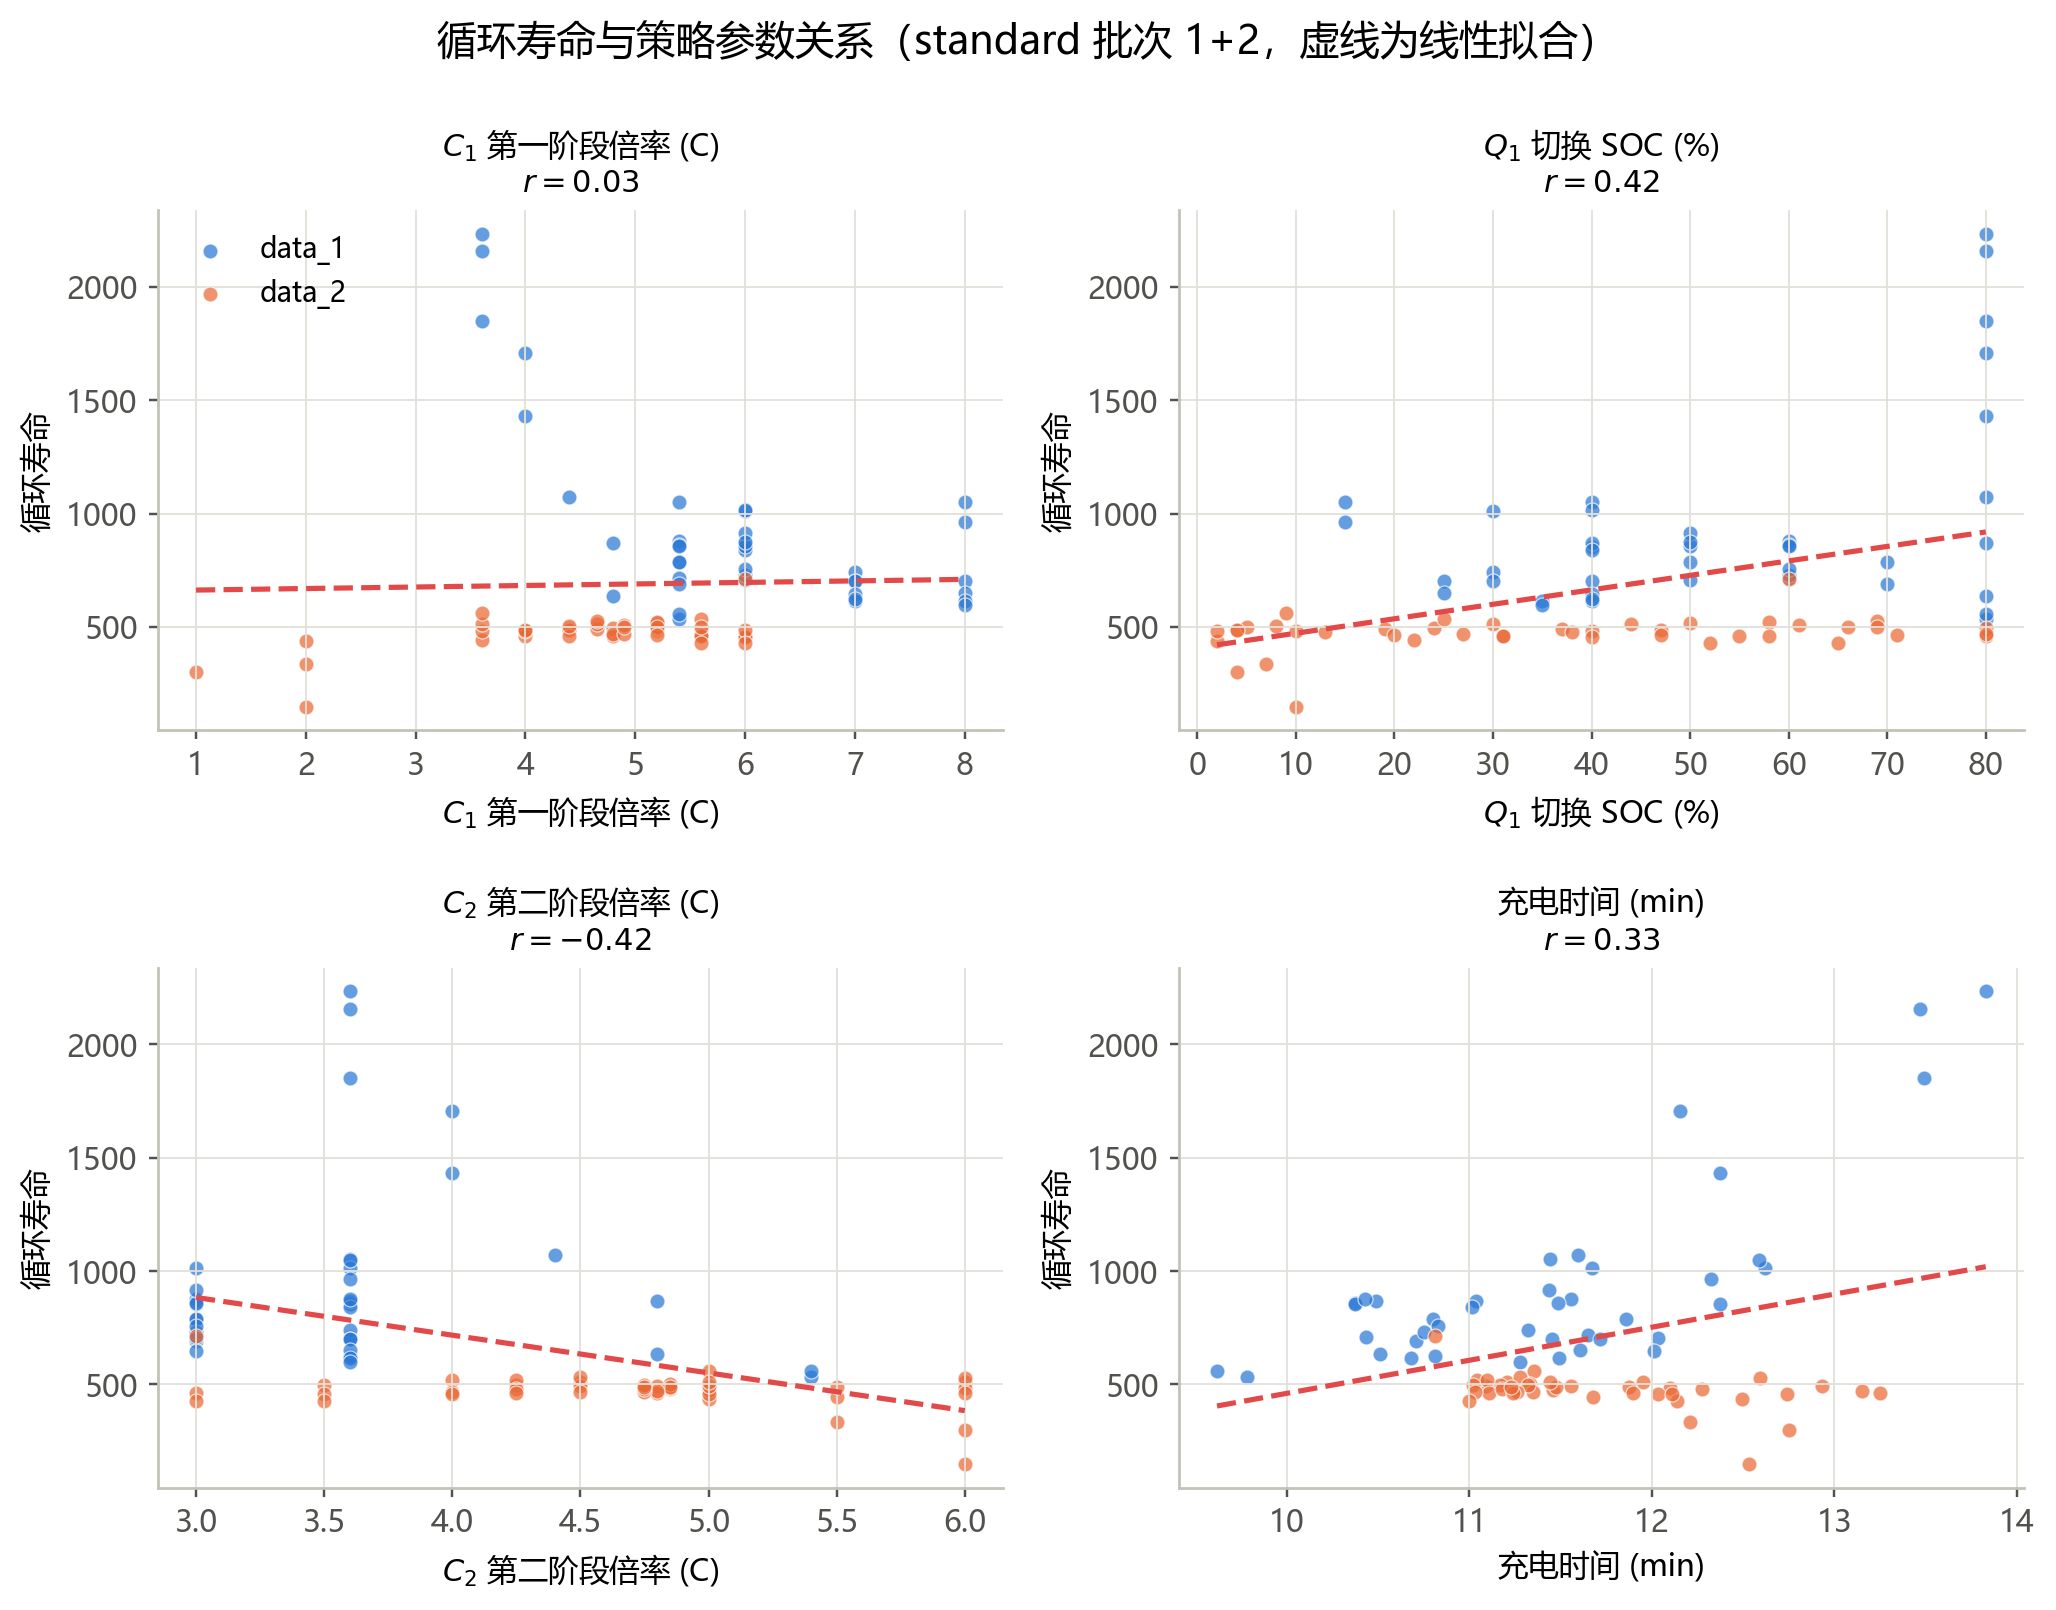
\includegraphics[width=0.95\textwidth]{figures/fig2.png}
\caption{cycle\_life 与各策略参数关系（standard 批次）}
\label{fig:fig2}
\end{figure}

\begin{enumerate}
\item \textbf{$C_2$ 是主要的负向倍率因素（$r=-0.418$）。}第二阶段充电覆盖从 $Q_1$ 到 80\% SOC 的中高电量区间，该区间内负极电位更接近析锂电位，高倍率充电会显著加剧负极析锂与电解液分解。短寿命策略（如 1C(4\%)-6C、2C(10\%)-6C）的共同特征正是 $C_2\ge5.5$C。
\item \textbf{$C_1$ 的影响较弱（$r=0.026$）。}第一阶段发生在低 SOC 区间，负极嵌锂位点充足、析锂风险低，短暂高倍率冲击可耐受。例如 8C(15\%)-3.6C 虽 $C_1$ 高达 8C，但因仅持续到 15\% SOC 即切换至温和的 3.6C，寿命仍达约 1000。需注意 $C_1$ 与 $Q_1$ 在批次 1 内存在实验设计混杂（$r=-0.88$），单变量相关不能完全反映 $C_1$ 的独立效应。
\item \textbf{$Q_1$ 的影响需结合 $C_1$ 解释。}$Q_1$ 决定高倍率第一阶段的作用时长。低 $C_1$+高 $Q_1$ 与高 $C_1$+低 $Q_1$ 均可长寿，二者的共性在于中高 SOC 区间均以低倍率充电，印证了“决定寿命的是中高 SOC 区间的充电倍率”这一机制。
\item \textbf{充电时间与寿命正相关（$r=0.330$）。}各策略充电至 80\% SOC 的时间差异不大（约 11$\sim$14 min），但充电时间更长的策略（通常倍率更温和）寿命更长；寿命差异达约 15 倍，说明决定寿命的关键是充电电流在 SOC 轴上的分布方式，而非单纯的快慢。
\end{enumerate}

\textbf{批次效应说明。}在控制策略参数后，批次 2 的寿命残差系统性为负（见第 6.6 节），表明批次间存在系统性环境/工艺差异（温控、夹具、批次一致性等）。故策略横向比较应优先采用同批次数据，跨批次结论需谨慎。

\subsection{参数相关性与数据探索}\label{sec:eda}

为刻画策略参数与寿命的整体关联结构，计算各参数间及与寿命的 Pearson 相关矩阵（图 \ref{fig:fig12}）。结果显示：$C_2$ 与寿命呈最强负相关（$r=-0.42$），$Q_1$ 与充电时间 $T_{80}$ 与寿命正相关（$r=0.42$ 与 $0.33$），而 $C_1$ 与寿命的相关较弱（$r=0.03$）。参数之间的相关性总体较弱（$|r|<0.4$），其中 $C_1$ 与 $Q_1$ 的整体相关仅 $0.03$，说明跨批次合并数据时各参数并非简单线性纠缠，其独立效应需依赖第 7 节的多变量回归解耦。但需注意，这一弱相关是跨批次合并的结果：在批次 1 内，$C_1$ 与 $Q_1$ 呈强负相关（$r=-0.88$），高 $C_1$ 策略普遍设置低 $Q_1$，因而批次 1 内难以独立识别二者的效应。这一"批次内局部混杂、跨批次整体正交"的结构，正是批次 1 与合并回归中 $C_1$、$Q_1$ 系数符号差异的原因，也进一步说明必须在多变量框架下结合批次效应建模。

图 \ref{fig:fig1} 的箱线图进一步显示：批次 2 的寿命分布整体下移（中位数 480）且跨度大，其中包含大量 $C_2\ge5$C 的激进攻略；批次 1 与批次 3 的寿命中位数接近（840 与 962），但分布形态不同。综合相关矩阵与分布特征可见，寿命差异主要由 $C_2$ 等策略参数系统驱动，而非随机噪声，这为后续定量建模提供了基础。

\begin{figure}[htbp]
\centering
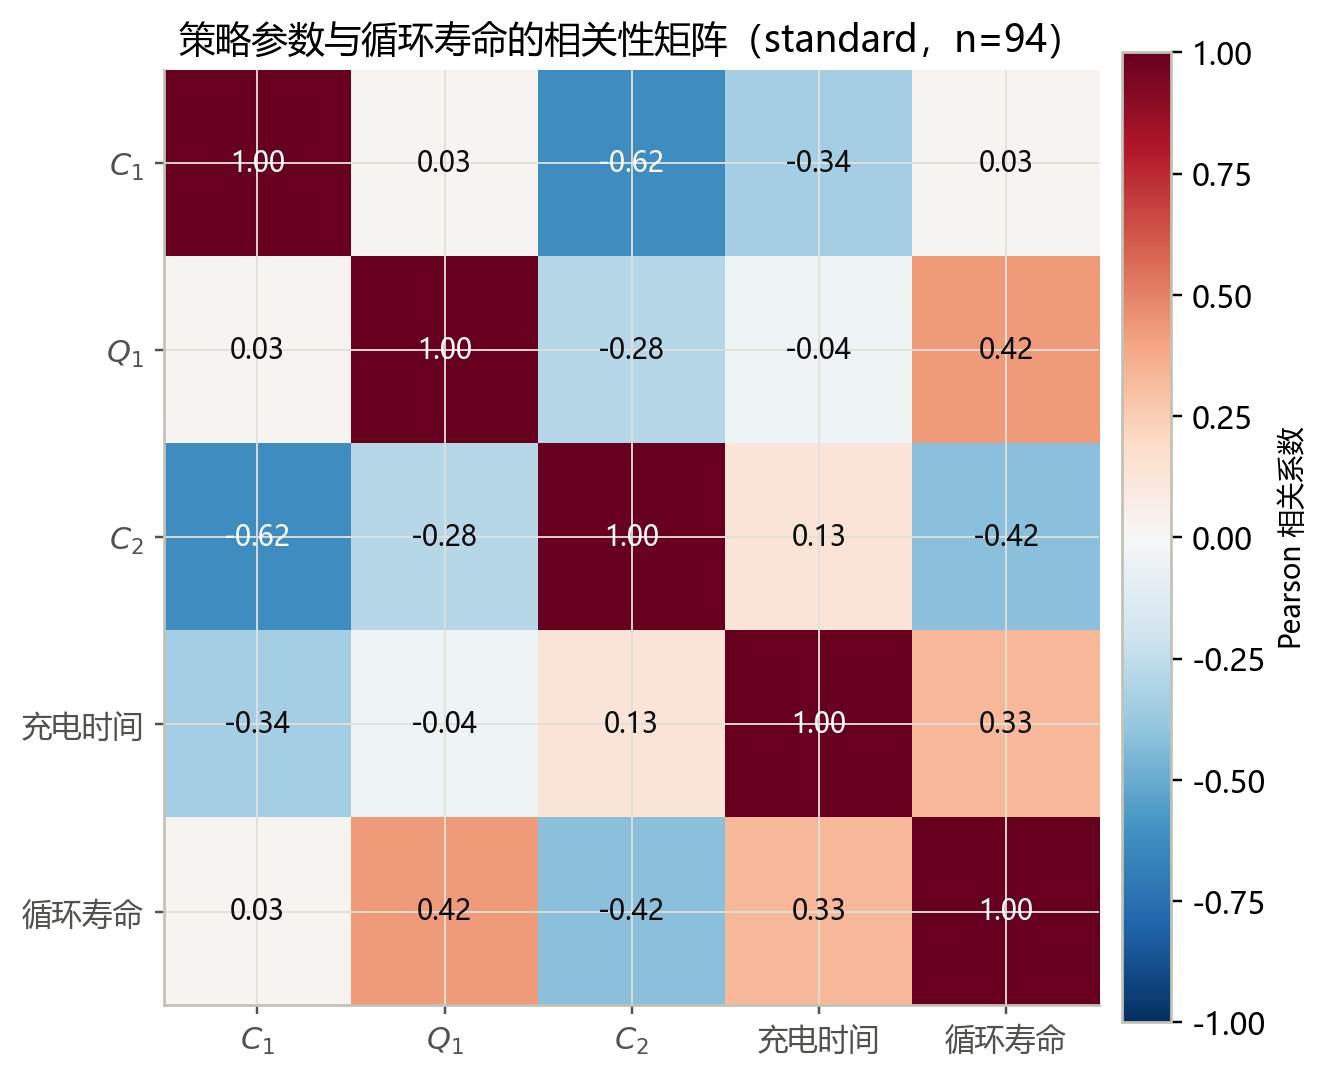
\includegraphics[width=0.72\textwidth]{figures/fig12.png}
\caption{策略参数与循环寿命的相关性矩阵（standard，n=84）}
\label{fig:fig12}
\end{figure}

\subsection{充电时间分析}\label{sec:charge-time}

问题一要求整理各电池的充电时间信息。图 \ref{fig:fig17}（左）显示充电时间随 $C_2$ 档位的分布：各档位充电时间中位数均在 11$\sim$14 min 之间，差异不大，说明"充电快慢"本身并非寿命差异的来源。图 \ref{fig:fig17}（右）将实测充电时间与理想物理模型（$T_{80}=60\cdot\frac{Q_1/100}{C_1}+60\cdot\frac{(80-Q_1)/100}{C_2}$）对比，可见大部分点落在 $y=x$ 附近，但在高倍率区（理想时间较短处）实测普遍略高于理想值，印证了电压限流造成的效率损失。这一分析为第 9 节充电时间模型的构建提供了数据基础。

\begin{figure}[htbp]
\centering
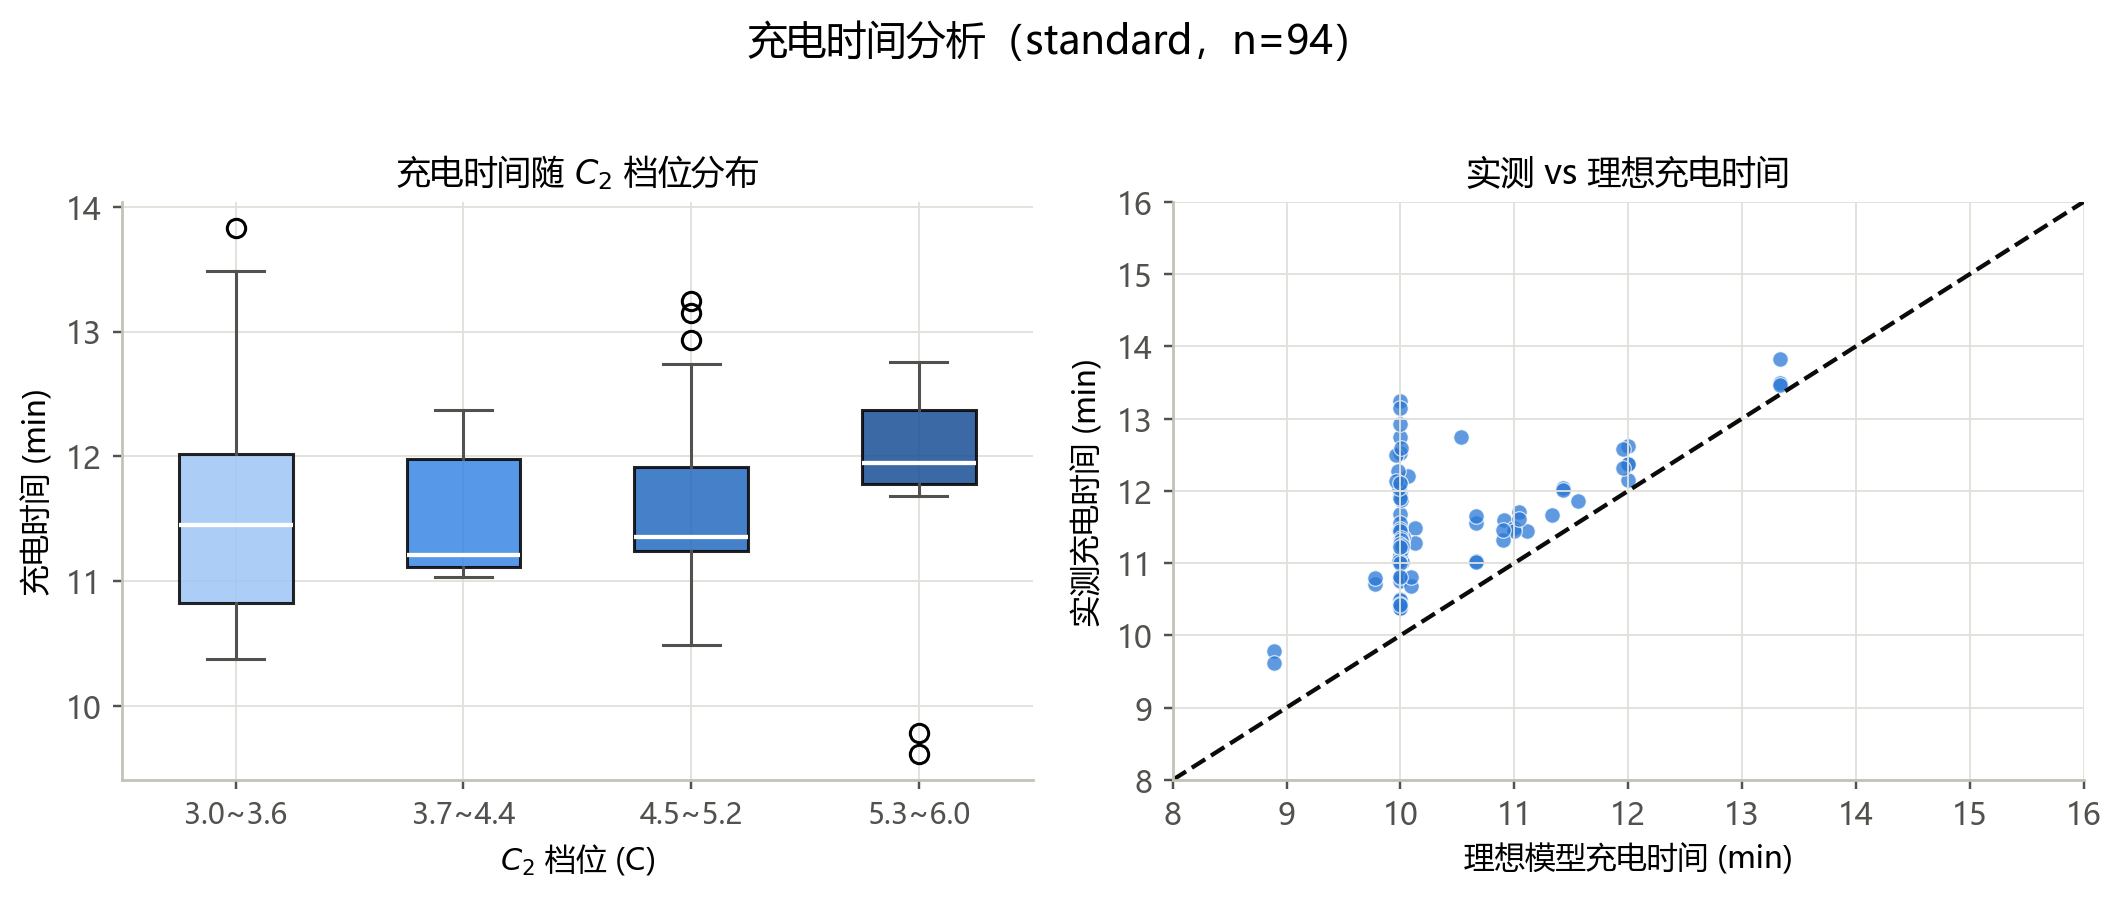
\includegraphics[width=0.92\textwidth]{figures/fig17.png}
\caption{充电时间分析：随 $C_2$ 档位分布与理想模型对比（standard，n=84）}
\label{fig:fig17}
\end{figure}

\subsection{批次效应可视化}

批次效应是本数据集的显著特征。为定量刻画在控制策略参数后批次间的残余差异，采用剂量模型（第 7.3 节）预测各电池寿命，并绘制实测寿命与模型预测之差的残差分布（图 \ref{fig:fig21}）。结果显示：批次 2 的寿命残差系统性为负（中位数显著低于零），即相同策略参数下批次 2 电池的实测寿命普遍低于模型预测，说明批次间存在系统性环境/工艺差异（温控、夹具、批次一致性等）。这一残余批次效应正是第 7.1 节回归中批次虚拟变量系数显著为负（$\beta=-0.11$）的来源。因此后文的策略比较一律在同批次内进行，跨批次结论仅作为相对参考。

\begin{figure}[htbp]
\centering
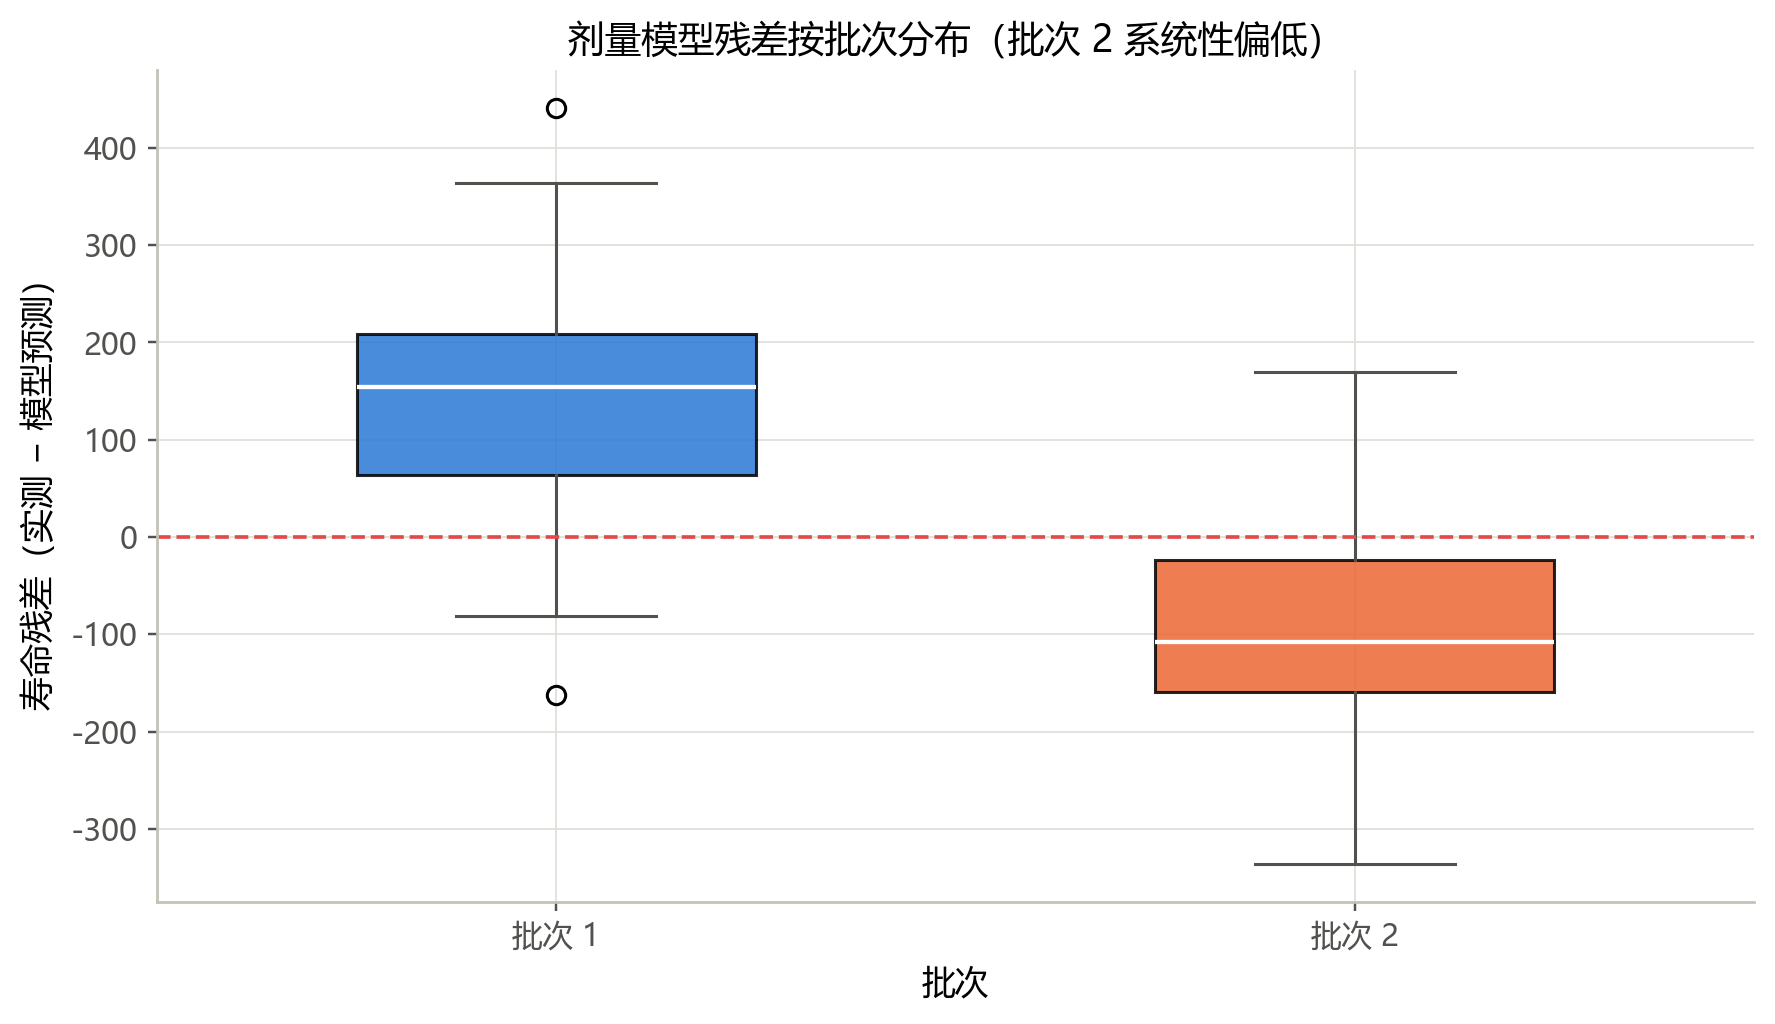
\includegraphics[width=0.68\textwidth]{figures/fig21.png}
\caption{剂量模型寿命残差按批次分布（批次 2 系统性偏低，批次效应）}
\label{fig:fig21}
\end{figure}

% ==================== 七、问题二 ====================
\section{问题二：充电策略参数对寿命衰减影响的量化模型}

\subsection{多变量回归模型}

基于 84 个 standard 电池，以 $\log_{10}$（循环寿命）为因变量，建立含批次效应的多变量线性回归：
\begin{equation}\label{eq:reg}
\log_{10}(L) = \beta_0 + \beta_1 C_1 + \beta_2 Q_1 + \beta_3 C_2 + \beta_4 T_{80} + \beta_5 \mathbb{1}_{\mathrm{batch2}} + \varepsilon.
\end{equation}
标准化（Z-score）回归结果见表 \ref{tab:reg}。模型 $R^2=0.674$（不含批次为 0.439），批次效应吸收了约 0.24 的 $R^2$。

\begin{table}[htbp]
\centering
\caption{多变量回归结果（含批次效应，$n=84$，$R^2=0.674$）}
\label{tab:reg}
\begin{tabular}{ccccc}
\toprule
变量 & 标准化系数 $\beta$ & 标准误 & $t$ & $p$ 值 \\
\midrule
$C_1$（第一阶段倍率） & $-0.021$ & 0.017 & $-1.28$ & 0.205 \\
$Q_1$（切换 SOC） & $+0.032$ & 0.013 & 2.49 & 0.015 \\
$C_2$（第二阶段倍率） & $-0.040$ & 0.017 & $-2.28$ & 0.025 \\
充电时间 $T_{80}$ & $+0.044$ & 0.013 & 3.43 & 0.001 \\
批次 2 效应 & $-0.116$ & 0.016 & $-7.50$ & $<0.0001$ \\
\bottomrule
\end{tabular}
\end{table}

未含批次效应的原始尺度模型为
\begin{equation}\label{eq:reg-raw}
\log_{10}(L) = 2.528 + 0.0005 C_1 + 0.0023 Q_1 - 0.0992 C_2 + 0.0497 T_{80},\quad R^2=0.439.
\end{equation}
结果显示：$C_2$ 每提高 1C，$\log_{10}$ 寿命约下降 0.099（寿命约衰减 20\%），为负向效应最显著的倍率参数；充电时间 $T_{80}$ 在控制 $C_2$ 后显著为正（偏相关 $+0.363$，充电越温和寿命越长）；$C_1$ 在含批次模型中不显著，源于批次 1 内其与 $Q_1$ 的实验设计混杂。

\subsection{各因素贡献排序与偏相关分析}

采用“留一变量 $R^2$ 变化”评估相对重要性（表 \ref{tab:imp}）。各策略参数的 $\Delta R^2$ 排序为：$T_{80}$（0.050）$>$ $Q_1$（0.026）$>$ $C_2$（0.022）$>$ $C_1$（0.007），批次效应占 0.235。偏相关系数（控制其余变量与批次）显示充电时间 $T_{80}$（$+0.363$）、$Q_1$（$+0.271$）与 $C_2$（$-0.250$）为最重要的策略维度（图 \ref{fig:fig4}）。

\begin{table}[htbp]
\centering
\caption{因素相对重要性（$\Delta R^2$ 与偏相关）}
\label{tab:imp}
\begin{tabular}{ccc}
\toprule
因素 & $\Delta R^2$ & 偏相关系数 \\
\midrule
批次 2 & 0.235 & $-0.647$ \\
充电时间 $T_{80}$ & 0.050 & $+0.363$ \\
$Q_1$ & 0.026 & $+0.271$ \\
$C_2$ & 0.022 & $-0.250$ \\
$C_1$ & 0.007 & $-0.143$ \\
\bottomrule
\end{tabular}
\end{table}

\begin{figure}[htbp]
\centering
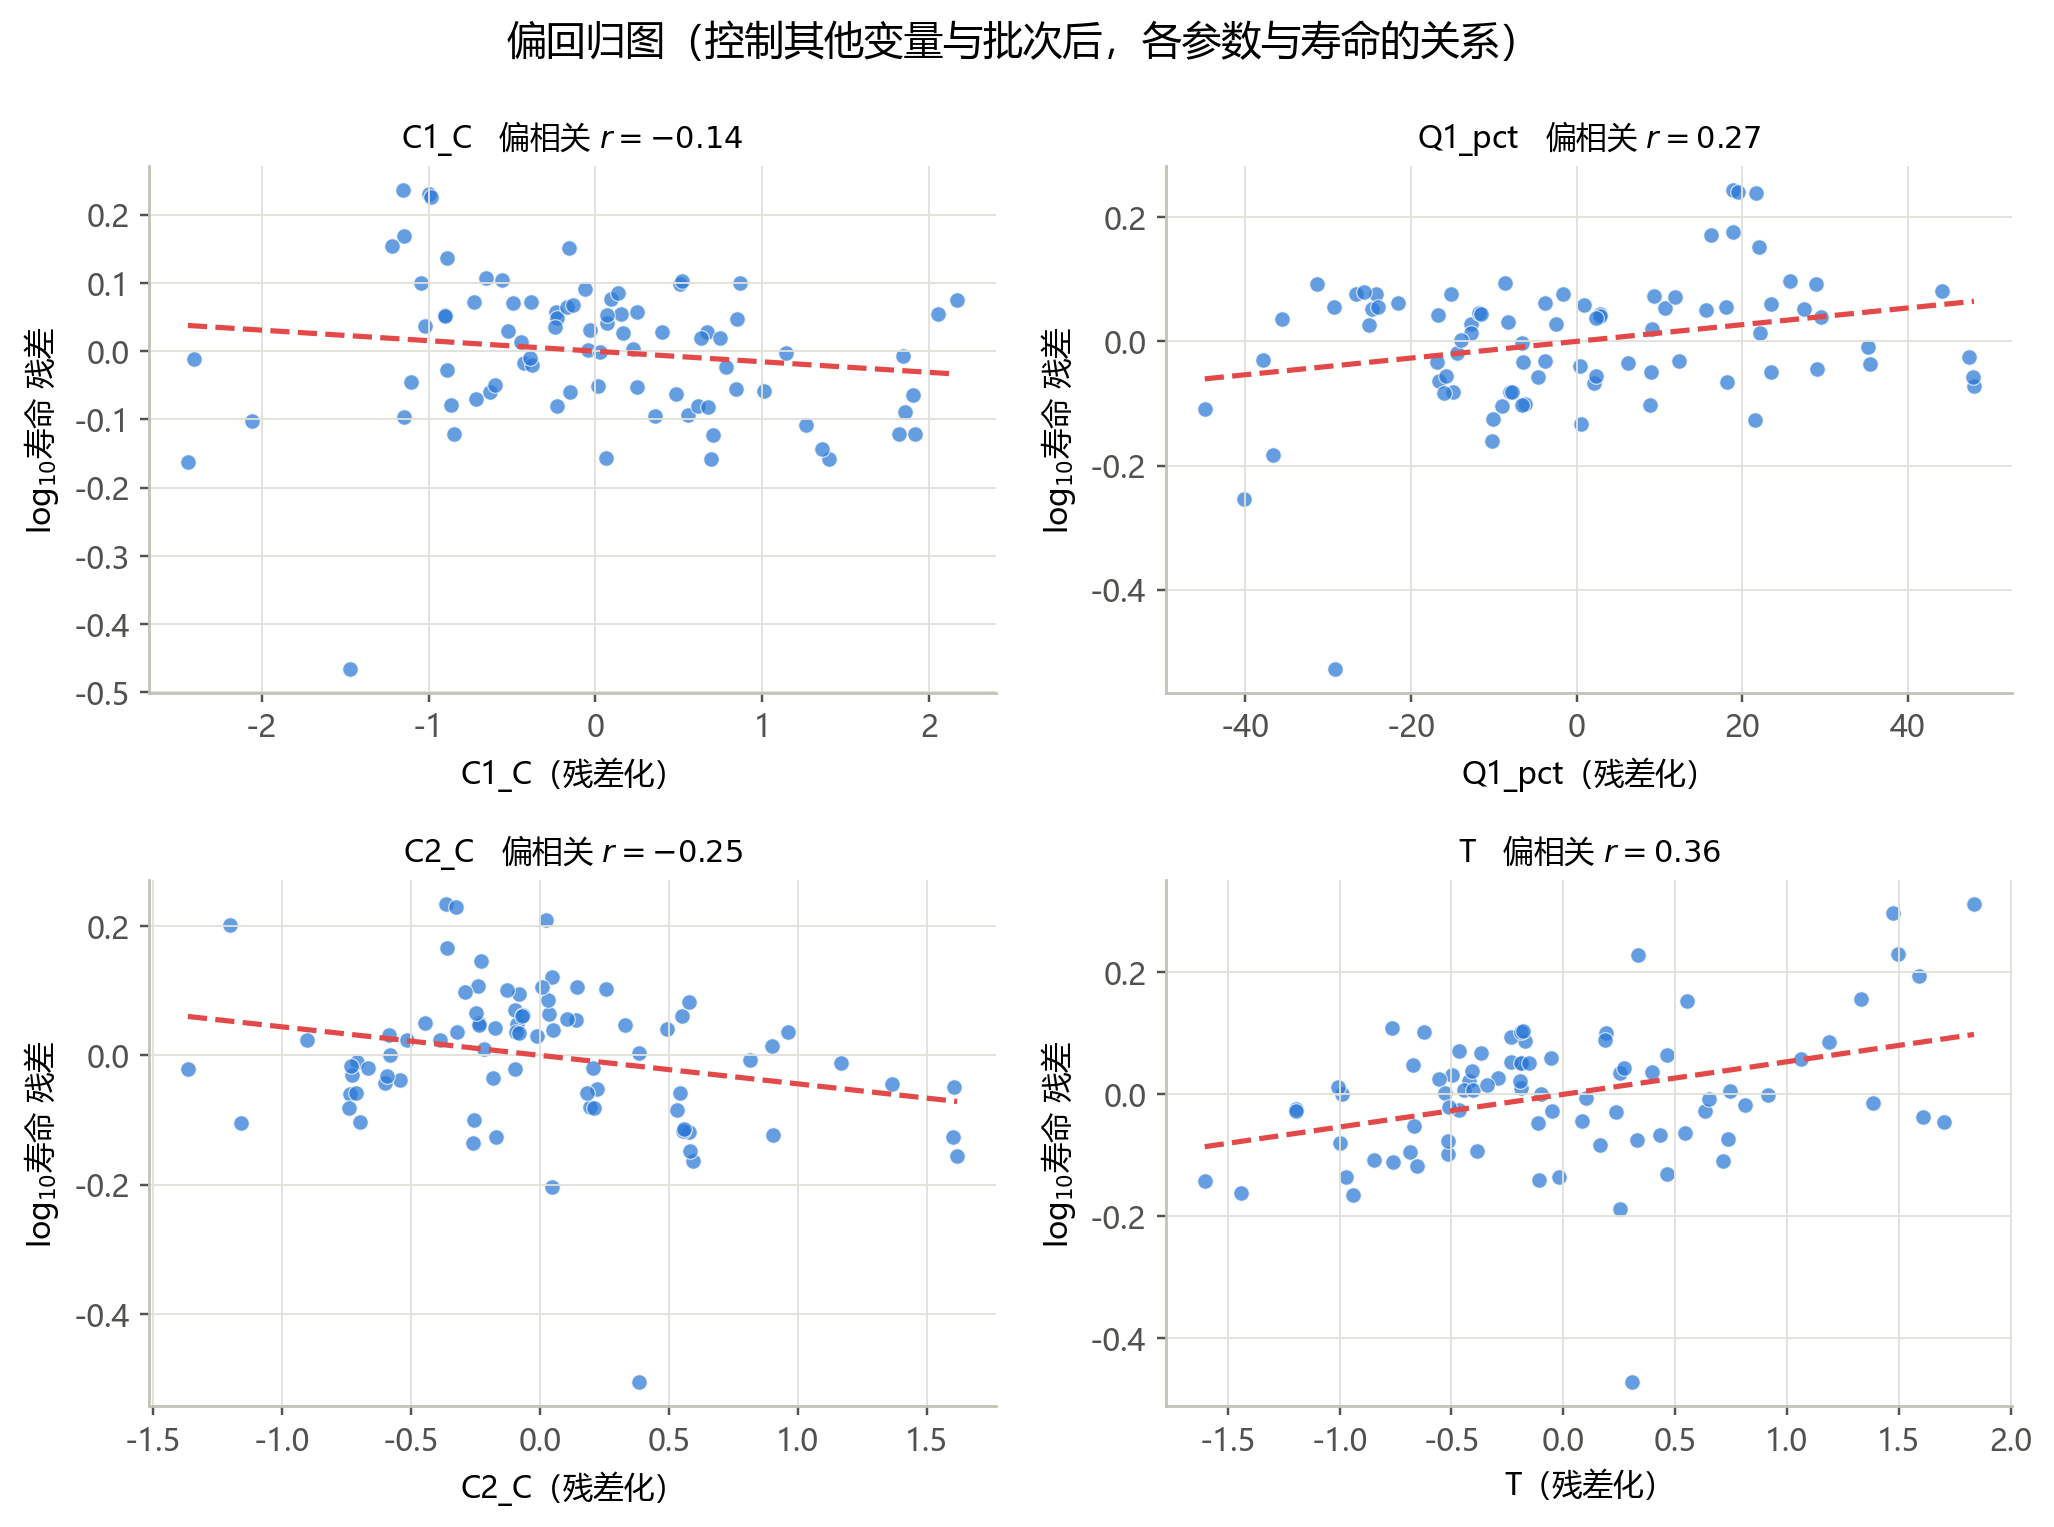
\includegraphics[width=0.9\textwidth]{figures/fig4.png}
\caption{偏回归图（控制其他变量与批次后，各参数与寿命的关系）}
\label{fig:fig4}
\end{figure}

从物理机制上解释上述排序：充电时间 $T_{80}$ 的偏相关最强（$+0.363$），反映"充电越温和（耗时越长）寿命越长"的整体效应——$T_{80}$ 由 $C_1$、$C_2$、$Q_1$ 共同决定，是充电激进程度的综合指示；$C_2$ 对应的第二阶段恰好覆盖负极最接近析锂电位的中高 SOC 区间，其偏相关显著为负（$-0.250$），说明高倍率充电是独立的寿命缩短因素；$Q_1$ 正相关（$+0.271$），反映切换点越靠后、中高 SOC 区间的高倍率暴露越短。$C_1$ 偏相关较弱，与低 SOC 区间析锂风险较低、且受批次 1 内参数范围限制有关。这一排序回答了问题二要求的"各因素影响程度排序"。

\subsection{不同 SOC 区间高倍率影响的差异（剂量模型）}\label{sec:dose}

为直接检验“不同 SOC 区间高倍率充电影响是否有差异”，定义两个高倍率电量剂量：
\begin{equation}\label{eq:dose}
m_1 = \frac{C_1\cdot Q_1}{100}\ \text{（低 SOC 区间剂量）},\qquad
m_2 = \frac{C_2\cdot (80-Q_1)}{100}\ \text{（中高 SOC 区间剂量）}.
\end{equation}
建立 $\log_{10}(L)\sim m_1+m_2$ 回归（表 \ref{tab:dose-reg}）。结果表明：两个剂量的系数均为显著负值，高倍率充电电量越多、寿命越短；且 $m_2$ 的单位伤害更大——原始系数 $m_2=-0.424$ vs $m_1=-0.367$，即在中高 SOC 区间每注入 1 Ah 高倍率电量的寿命损伤比低 SOC 区间高约 16\%；模型 $R^2=0.635$，显著高于单变量相关所能解释的部分。策略参数空间上的寿命响应面见图 \ref{fig:fig5}。

从电化学机理看，这一"区间差异"源于负极析锂风险随 SOC 的非单调变化：低 SOC 区间负极电位较高、嵌锂位点充足，析锂过电位裕度大，短暂高倍率冲击造成的锂沉积与电解液副反应有限；而中高 SOC 区间负极表面锂浓度接近饱和，析锂电位窗口收窄，相同的高倍率电量注入会显著加剧析锂与 SEI 膜生长。因此，$m_1$、$m_2$ 系数之比（约 1.16）定量刻画了"同一安时数的高倍率电量，在 SOC 轴上的位置决定了其对寿命的伤害程度"。该剂量模型为后续优化提供了清晰的物理依据：**应尽量将高倍率充电安排在低 SOC 区间，而中高 SOC 区间保持温和倍率**。

\begin{table}[htbp]
\centering
\caption{SOC 剂量模型回归（$n=84$）}
\label{tab:dose-reg}
\begin{tabular}{cccc}
\toprule
变量 & 原始系数 & 标准化系数 $\beta$ & $p$ 值 \\
\midrule
截距 & 4.312 & --- & --- \\
$m_1$（低 SOC 剂量） & $-0.367$ & $-0.434$ & $<0.0001$ \\
$m_2$（中高 SOC 剂量） & $-0.424$ & $-0.519$ & $<0.0001$ \\
\bottomrule
\end{tabular}
\end{table}

\begin{figure}[htbp]
\centering
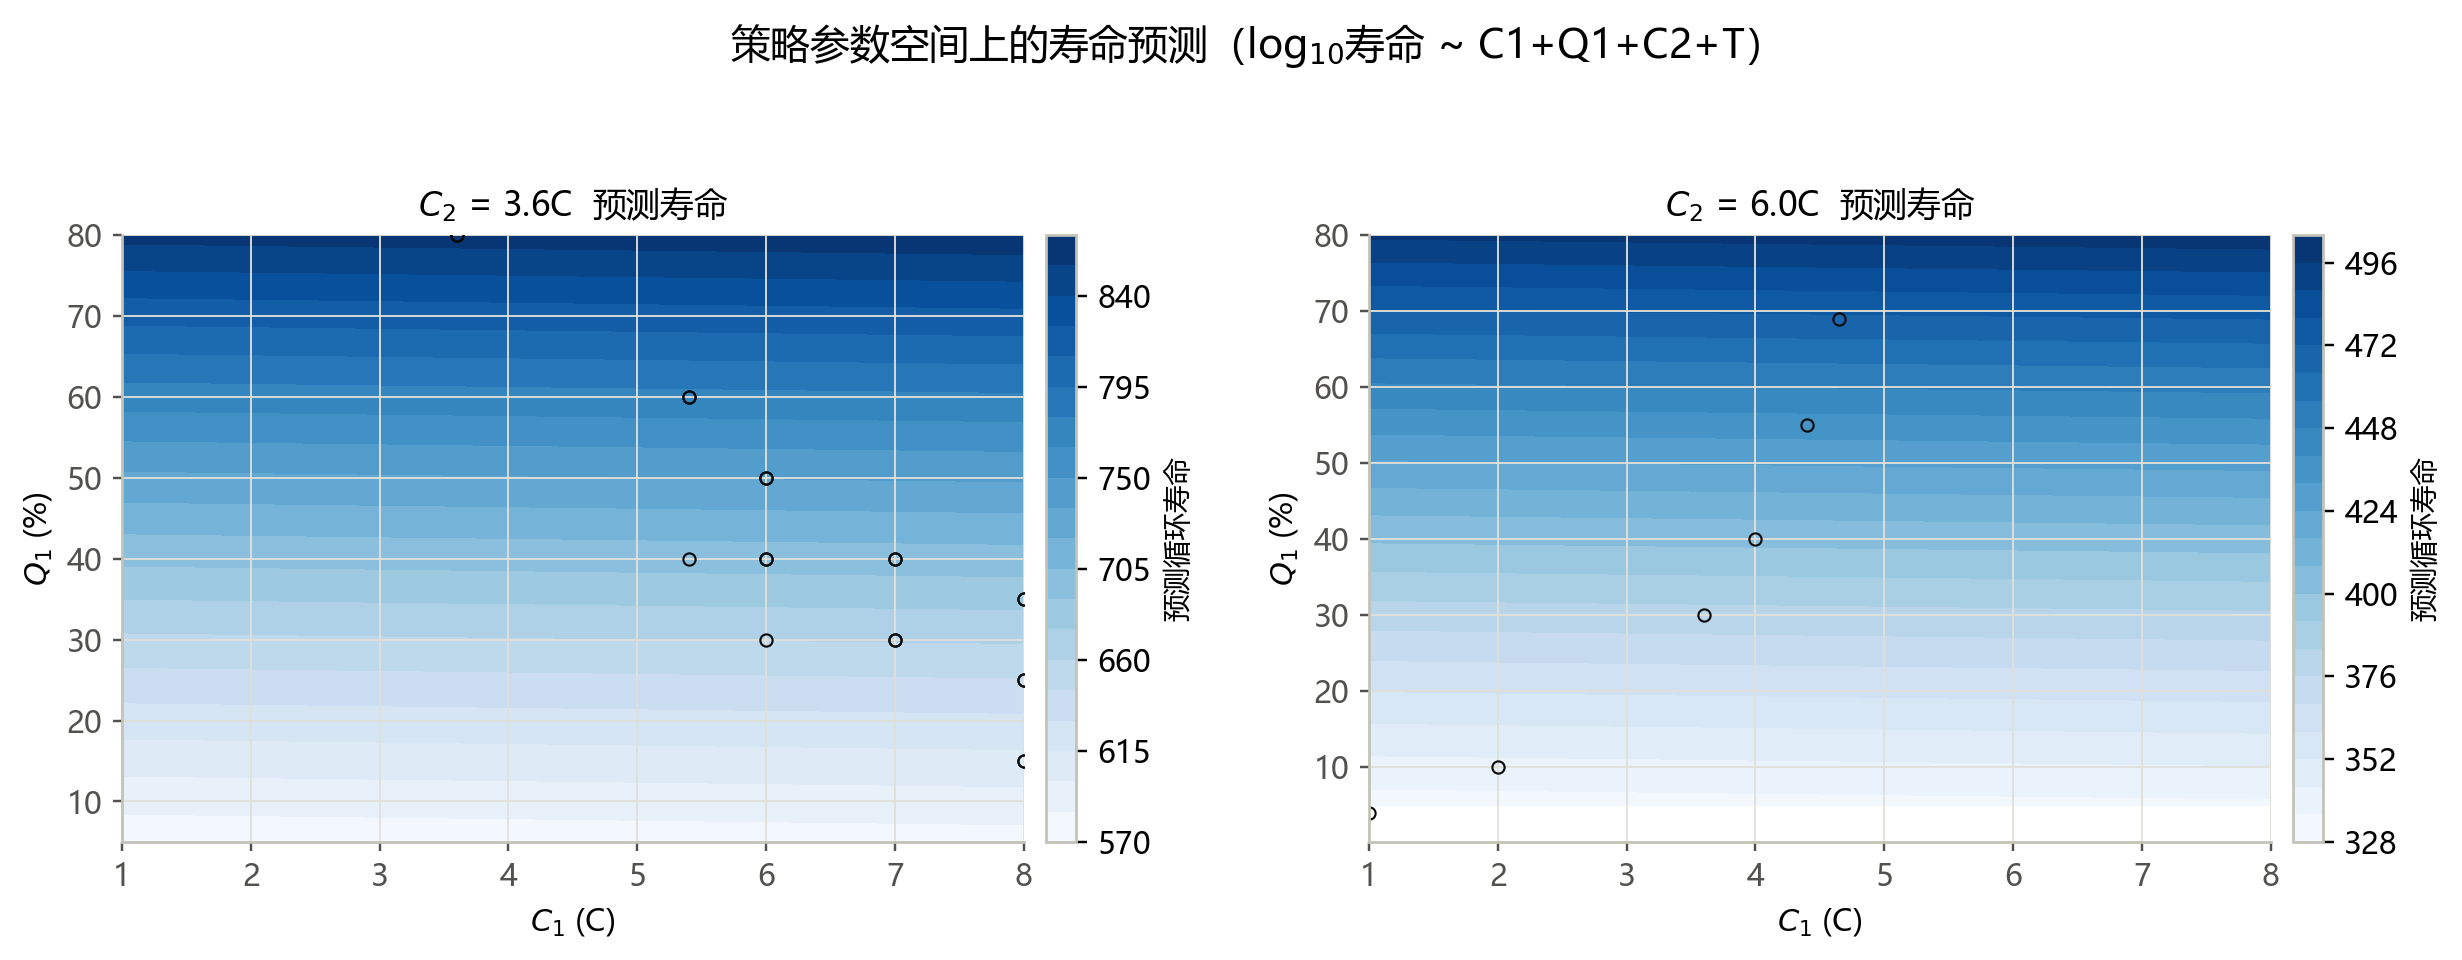
\includegraphics[width=0.95\textwidth]{figures/fig5.png}
\caption{策略参数空间上的寿命预测（$C_2=3.6$ 与 6.0C 响应面）}
\label{fig:fig5}
\end{figure}

\subsection{交互作用分析}

在回归中引入交互项（表 \ref{tab:interact}）：$C_1\times Q_1$ 为负（$-0.0042$），反映低 SOC 高倍率剂量的累积伤害；$C_2\times Q_1$ 为正（$+0.0046$），因 $Q_1$ 越大、第二阶段覆盖区间（$80-Q_1$）越小、$C_2$ 暴露越短，从交互角度印证 $C_2$ 的伤害与其中高 SOC 覆盖量成正比。

\begin{table}[htbp]
\centering
\caption{交互项回归（$n=84$，$R^2=0.626$）}
\label{tab:interact}
\begin{tabular}{ccc}
\toprule
变量 & 系数 & $p$ 值 \\
\midrule
$C_1$ & $+0.007$ & 0.683 \\
$Q_1$ & $-0.001$ & 0.872 \\
$C_2$ & $-0.426$ & $<0.0001$ \\
充电时间 $T_{80}$ & $-0.032$ & 0.053 \\
$C_1\times Q_1$ & $-0.0042$ & $<0.0001$ \\
$C_2\times Q_1$ & $+0.0046$ & $<0.0001$ \\
\bottomrule
\end{tabular}
\end{table}

交互项的结果可以统一到剂量视角理解：$C_1\times Q_1$ 项恰为 $m_1=C_1Q_1/100$ 的常数倍（忽略归一化），其负系数说明"低 SOC 区间高倍率电量的总注入量"越大、寿命越短；$C_2\times Q_1$ 项与 $m_2=C_2(80-Q_1)/100$ 互补——$Q_1$ 增大使 $m_2$ 减小，故 $C_2\times Q_1$ 系数为正。因此，交互项模型与第 7.3 节的剂量模型在机理上自洽，从"参数"与"剂量"两个视角交叉验证了同一结论。

\subsection{批次内稳健性}

分批次回归（表 \ref{tab:within-batch}）：批次 1 内 $C_1$、$Q_1$ 显著为负（该批次 $C_2$ 多在 3.0$\sim$3.6C、变化小，$C_2$ 效应不被识别），说明在 $C_2$ 温和前提下，延长第一阶段高倍率（增大 $C_1$ 或 $Q_1$）同样缩短寿命；批次 2 内策略空间集中于较高 $C_2$，$C_2$ 效应亦不被识别。因此，在完整策略参数空间中 $C_2$、$Q_1$、$T_{80}$ 的效应（表 \ref{tab:reg}）主导；在 $C_2$ 固定温和的批次内，$C_1$、$Q_1$ 成为主要调节因素。

\begin{table}[htbp]
\centering
\caption{批次内标准化回归系数}
\label{tab:within-batch}
\begin{tabular}{cccccc}
\toprule
批次 & $C_1$ & $Q_1$ & $C_2$ & $R^2$ & $n$ \\
\midrule
data\_1 & $-0.221^{\ast\ast\ast}$ & $-0.141^{\ast\ast\ast}$ & $-0.006$ & 0.630 & 41 \\
data\_2 & $+0.057^{\ast}$ & $+0.003$ & $+0.007$ & 0.329 & 43 \\
\bottomrule
\end{tabular}
\end{table}
注：$\ast\ast\ast$ 表示 $p<0.0001$，$\ast$ 表示 $p<0.01$。

\subsection{$C_2$ 档位效应与非线性考察}

将 $C_2$ 按档位分组考察寿命分布（图 \ref{fig:fig16}）：当 $C_2\le3.6$C 时寿命中位数为 815；当 $C_2$ 升至 $3.7\sim4.4$C 时降至 490，$4.5\sim5.2$C 与 $5.3\sim6.0$C 档位亦稳定在 485 左右。这一"先陡降、后趋平"的模式表明，$C_2$ 的伤害具有明显阈值特征——超过约 3.6C 后，继续升高倍率带来的额外寿命损失边际递减。这与回归中 $C_2$ 系数显著为负的线性结论方向一致，同时提示 $C_2$ 对寿命的影响可能存在非线性，策略优化应优先将 $C_2$ 控制在 3.6C 以内，这也为第 9 节的推荐策略提供了依据。

\begin{figure}[htbp]
\centering
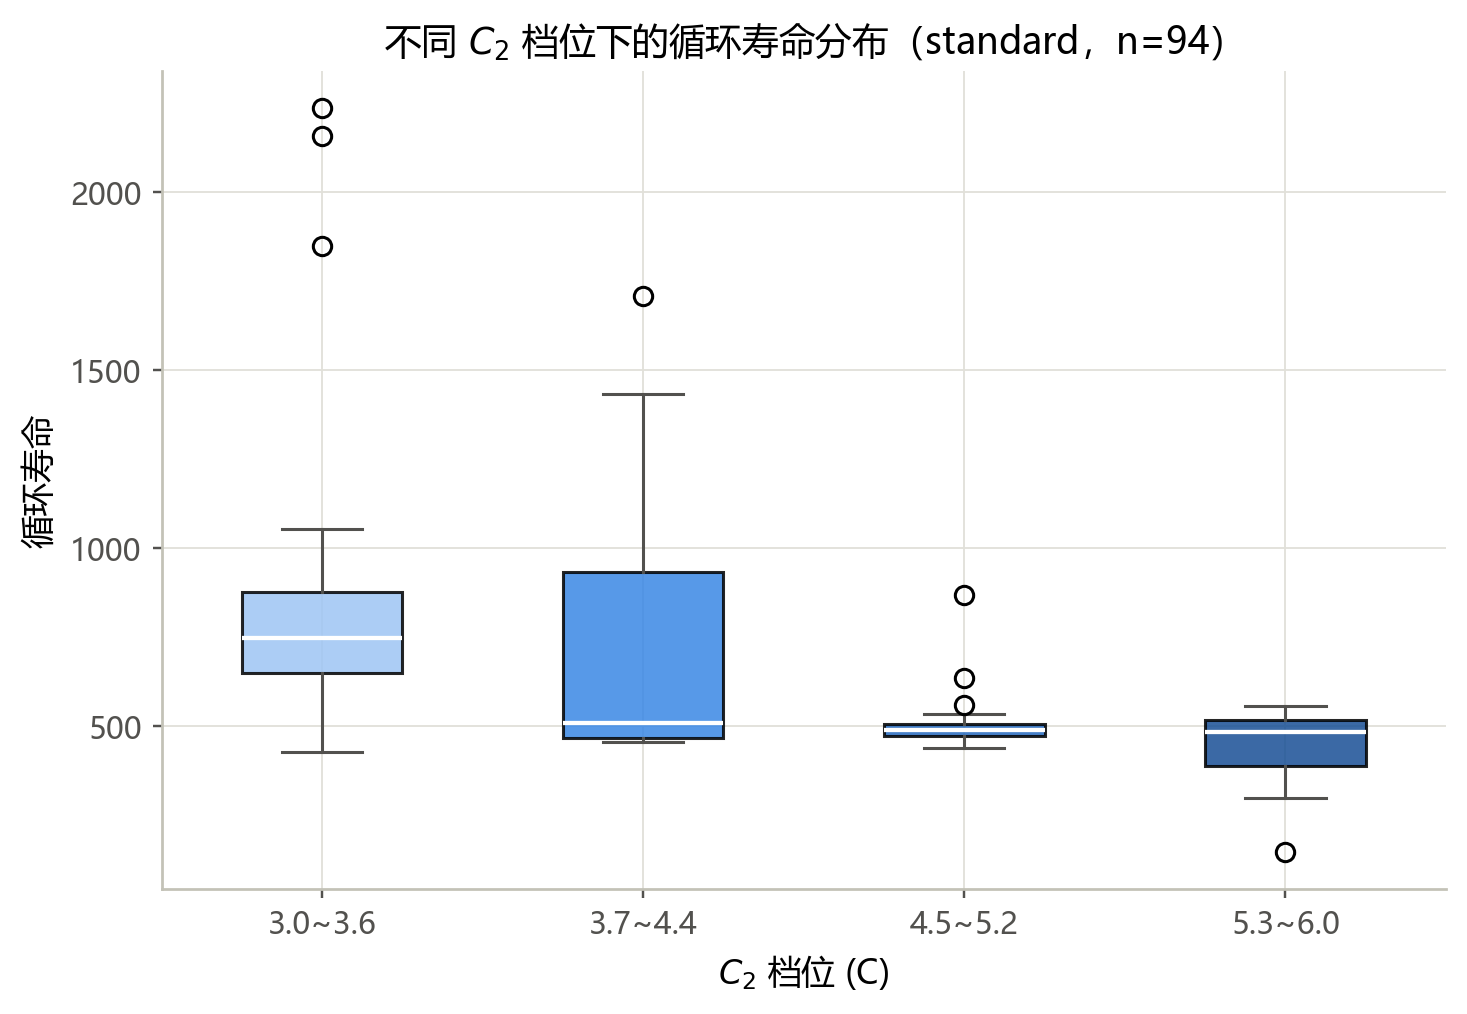
\includegraphics[width=0.7\textwidth]{figures/fig16.png}
\caption{不同 $C_2$ 档位下的循环寿命分布（standard，n=84）}
\label{fig:fig16}
\end{figure}

\subsection{回归模型残差诊断}

为检验第 7.1 节回归模型的有效性，进行残差诊断（图 \ref{fig:fig18}）。残差对拟合值散点随机分布在零线两侧、无明显的漏斗形或曲线趋势，说明模型不存在显著的异方差或非线性误设；残差直方图近似正态且以零为中心，表明模型无系统性偏差，主要误差来源为电池个体差异。这一诊断保证了第 8 节寿命预测与第 9 节策略优化所依赖的回归结论是可靠的。

\begin{figure}[htbp]
\centering
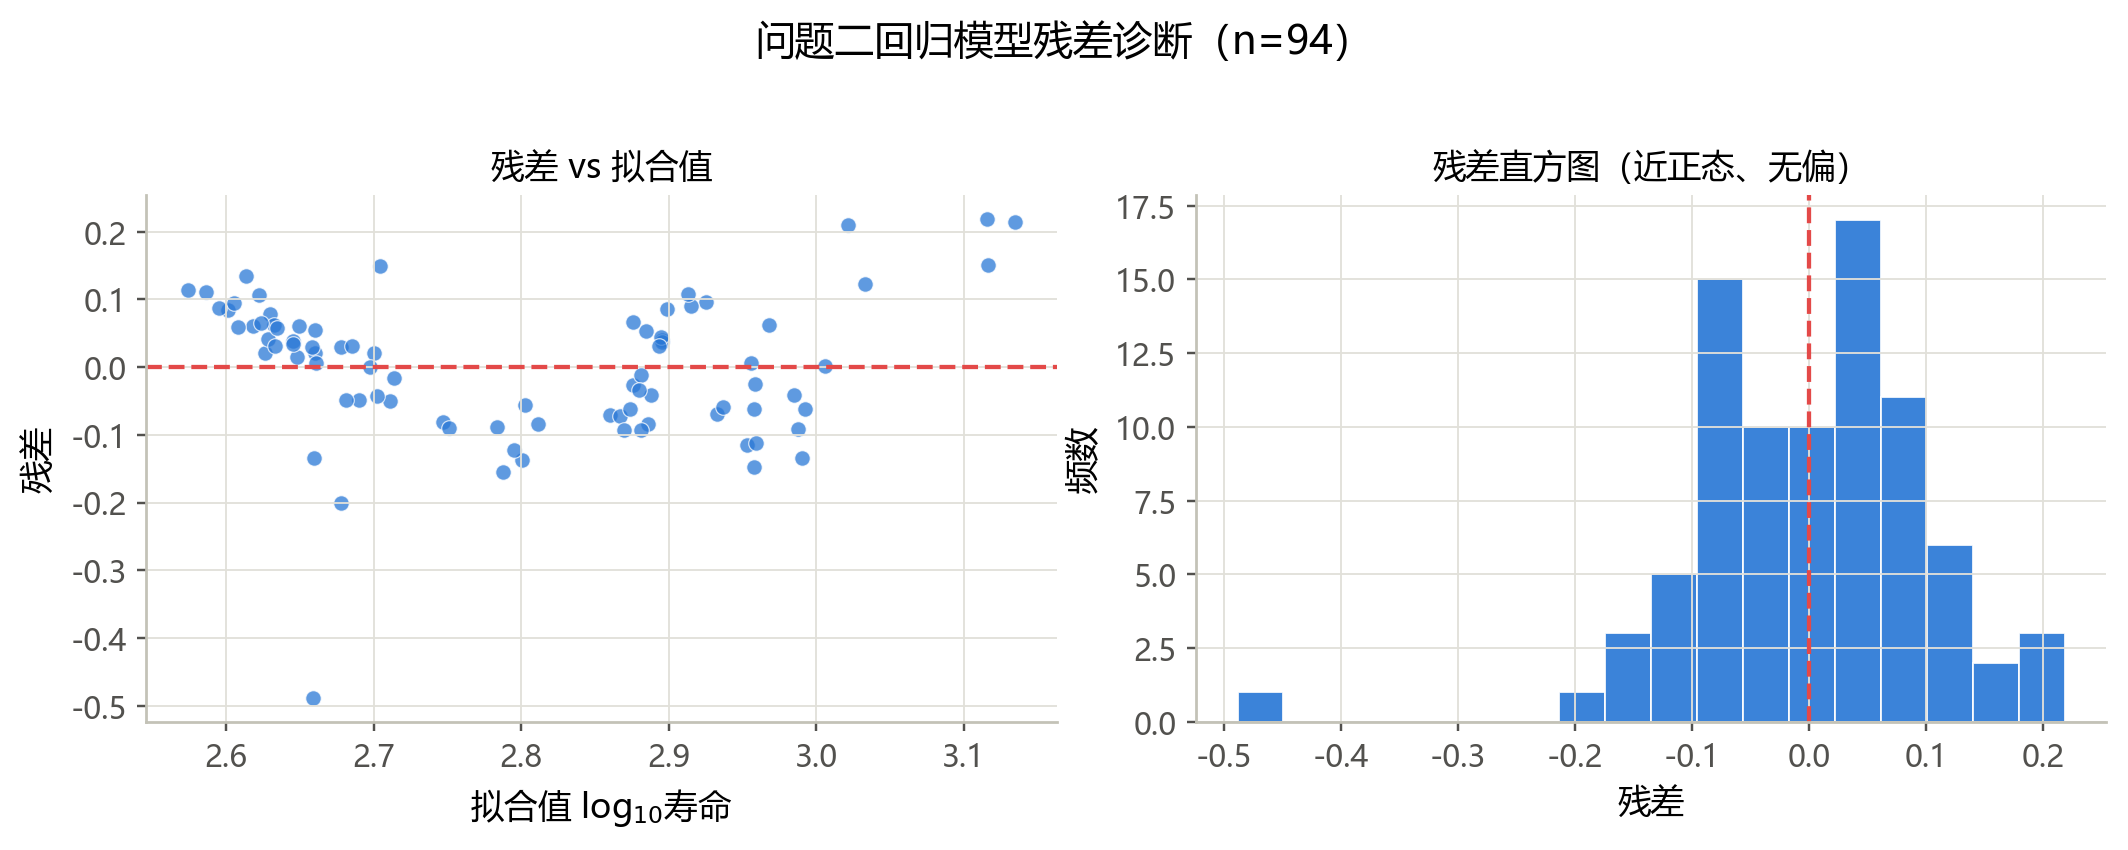
\includegraphics[width=0.92\textwidth]{figures/fig18.png}
\caption{问题二回归模型残差诊断（n=84）}
\label{fig:fig18}
\end{figure}

% ==================== 八、问题三 ====================
\section{问题三：基于早期循环数据的寿命预测模型}

\subsection{特征提取}

基于逐循环放电容量（Qd）、SOH 与充电时间序列，对每个电池在前 $k$ 个循环窗口（$k=5/10/20/50/100$）内提取三类特征：
\begin{enumerate}
\item \textbf{早期衰减特征}：$k$ 处 SOH（$SOH_k$）与容量损失（$100-SOH_k$）、SOH 线性拟合斜率及其 $R^2$、SOH/容量残差与一阶差分标准差、容量斜率；
\item \textbf{充电时间特征}：首循环充电时间、$k$ 处充电时间、充电时间斜率、一阶差分标准差与漂移量；
\item \textbf{潜伏时间特征}：SOH 首次低于阈值（99.9/99.8/$\cdots$/96\%）的循环序号（窗口内未达到则记截断值）。
\end{enumerate}
另将策略参数（$C_1,Q_1,C_2$、平均充电时间）作为可用特征，用于消融分析。

为说明"早期数据中已包含寿命信息"，图 \ref{fig:fig19} 展示了不同寿命特征电池前 60 个循环的 SOH 演化。可见即便在早期，长寿命电池与短寿命电池的 SOH 水平与波动幅度已呈现系统差异：短寿命电池（1C(4\%)-6C）的早期 SOH 已明显低于长寿命电池，且波动更大。这正是早期特征能够预测寿命的根本原因。

\begin{figure}[htbp]
\centering
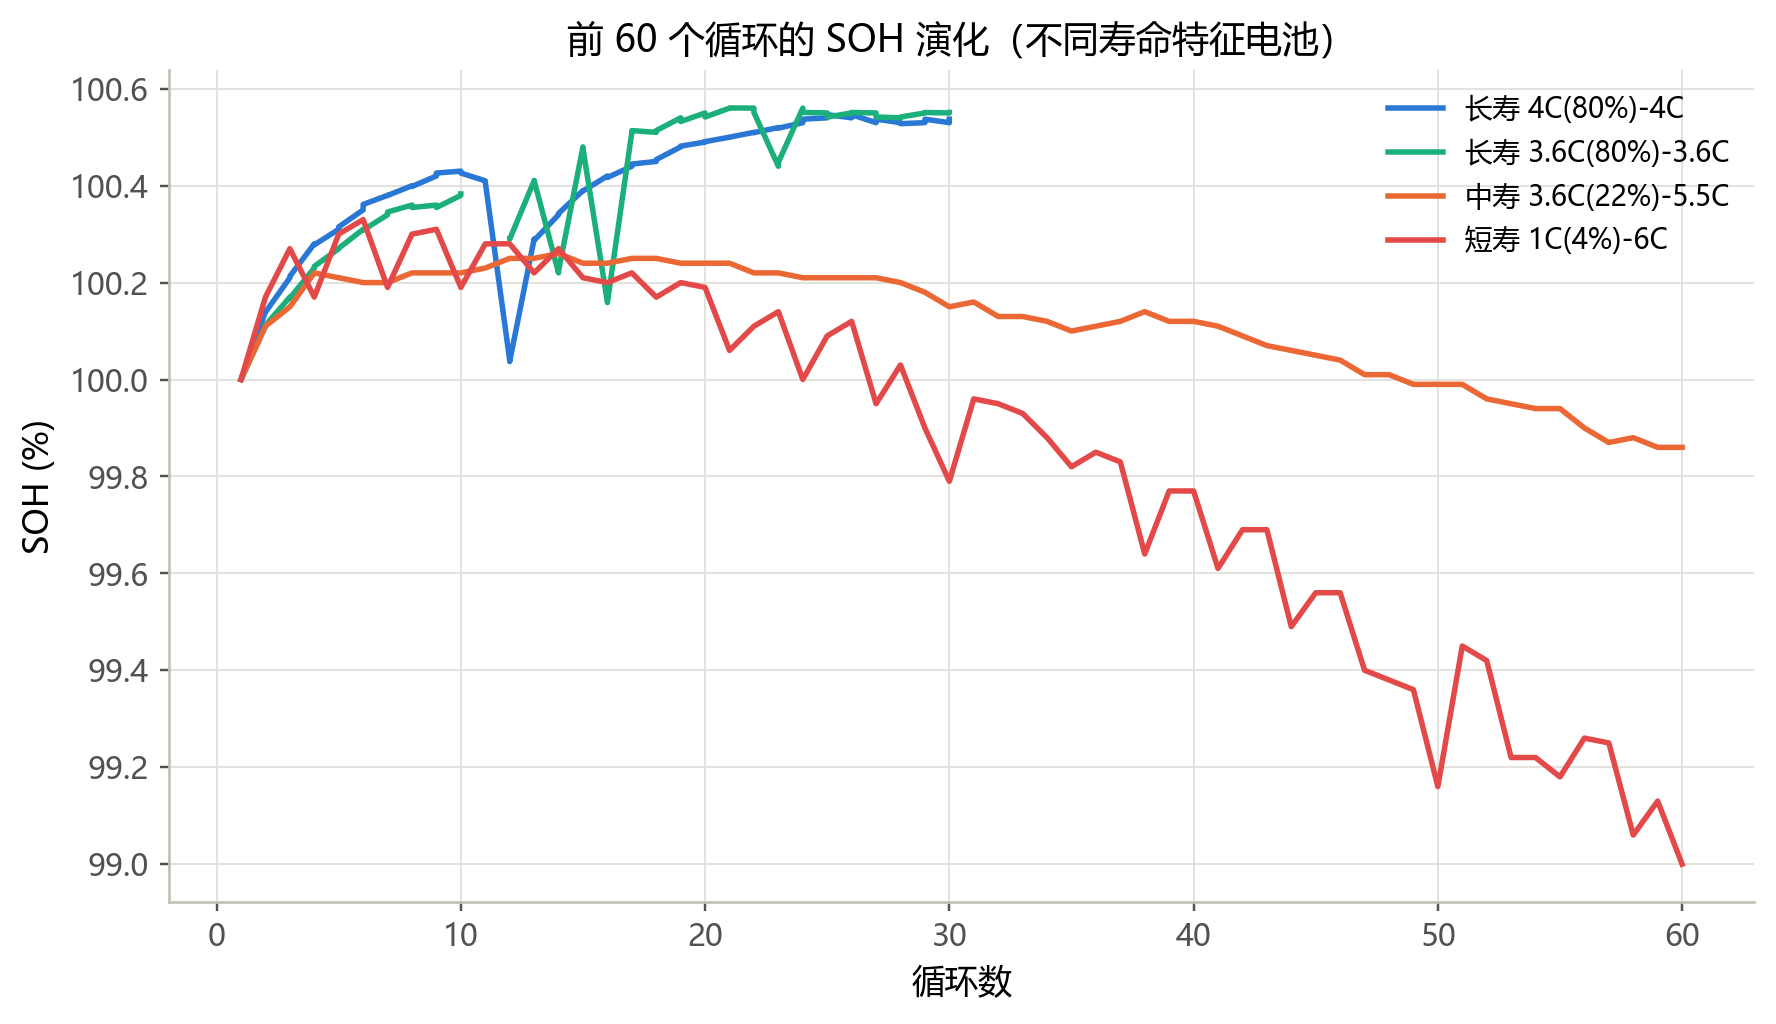
\includegraphics[width=0.72\textwidth]{figures/fig19.png}
\caption{前 60 个循环的 SOH 演化（不同寿命特征电池）}
\label{fig:fig19}
\end{figure}

\subsection{预测模型与评估方法}

以 $\log_{10}$（循环寿命）为目标，比较三种模型：Ridge 回归、随机森林（RF）与梯度提升回归树（GBM）。采用 5 折$\times$8 次重复交叉验证，以平均绝对百分比误差（MAPE，基于反变换寿命）与 $\log_{10}$ 尺度 $R^2$ 评价。三种模型的对比（表 \ref{tab:window}）显示，GBM 在各窗口下的 MAPE 均低于或接近 Ridge 与 RF，这是因为 GBM 能自适应地刻画特征间的非线性交互（例如充电时间漂移与 SOH 波动对寿命的联合作用），且对早期特征中的少量异常值鲁棒。故后续以 GBM 作为主预测模型。

\subsection{不同早期窗口长度的影响}

表 \ref{tab:window} 与图 \ref{fig:fig7} 给出各窗口的预测精度。随早期数据从 5 循环增加到 20 循环，GBM 的 MAPE 由 16.5\% 降至 15.3\%；继续增至 100 循环，Ridge 可降至 14.5\%、GBM 约 15.0\%，改善有限。$k=20$ 为预测精度与数据成本的良好折衷。

\begin{table}[htbp]
\centering
\caption{不同早期窗口长度下的预测误差（5 折$\times$8 重复 CV）}
\label{tab:window}
\begin{tabular}{ccccc}
\toprule
窗口 $k$ & Ridge MAPE(\%) & RF MAPE(\%) & GBM MAPE(\%) & GBM $R^2$ \\
\midrule
5 & 15.7 & 18.4 & 16.5 & 0.740 \\
10 & 22.6 & 17.8 & 17.1 & 0.738 \\
20 & 15.8 & 16.4 & 15.3 & 0.768 \\
50 & 16.5 & 15.9 & 15.3 & 0.771 \\
100 & 14.5 & 16.6 & 15.0 & 0.775 \\
\bottomrule
\end{tabular}
\end{table}

\begin{figure}[htbp]
\centering
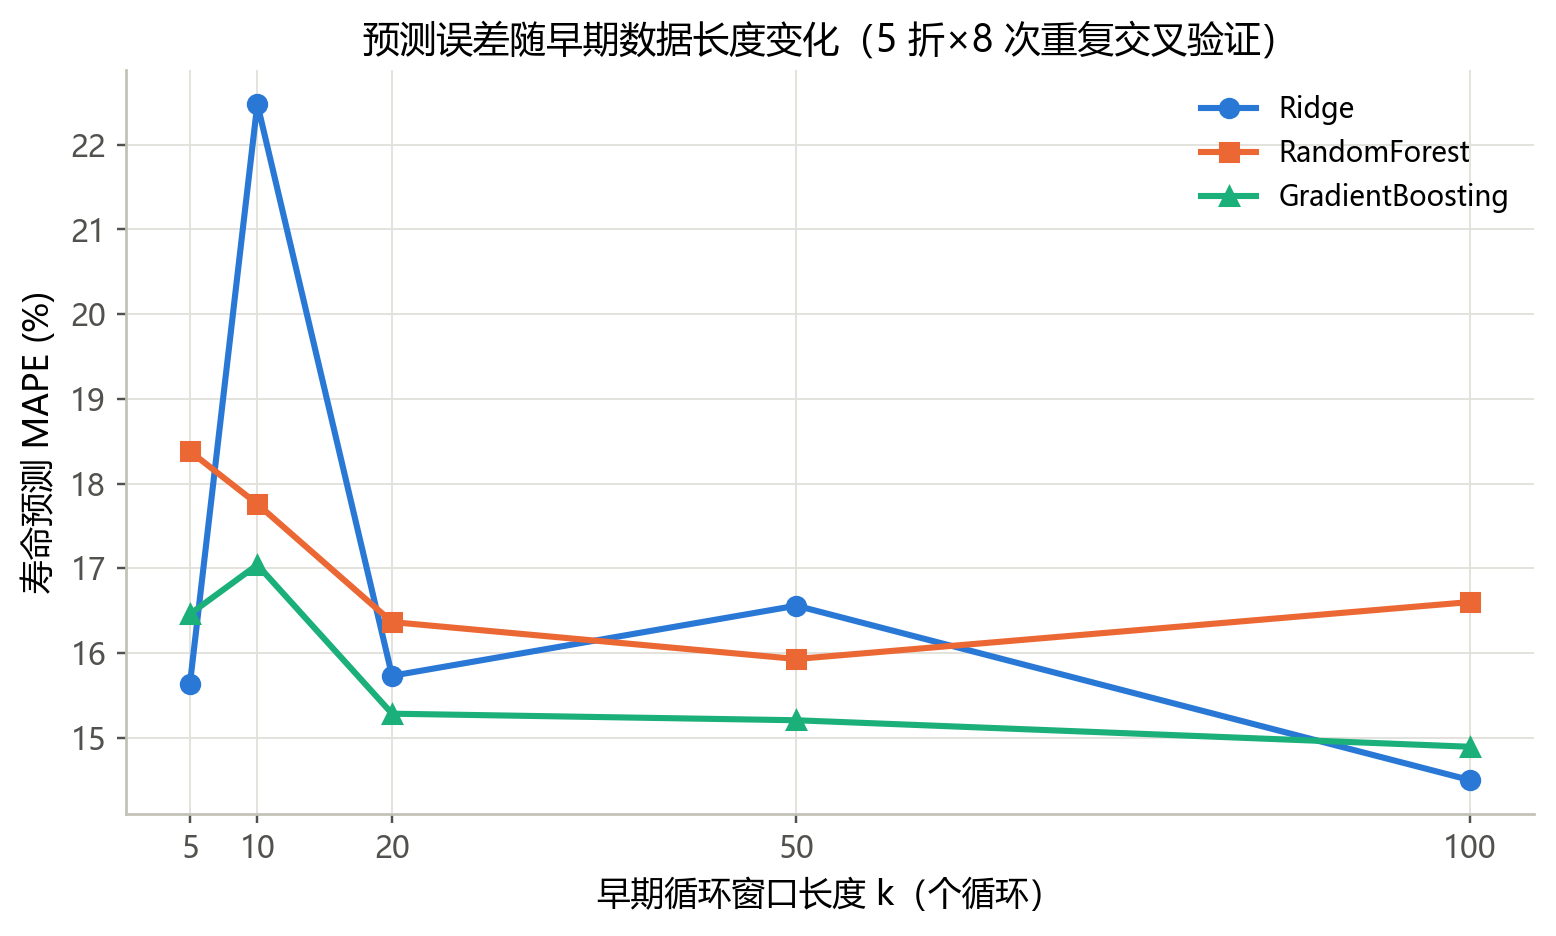
\includegraphics[width=0.75\textwidth]{figures/fig7.png}
\caption{预测误差随早期数据长度变化}
\label{fig:fig7}
\end{figure}

$k=100$ 时 GBM 的交叉验证预测--实测散点见图 \ref{fig:fig6}：绝大多数样本落在 $\pm10\%$ 误差带内，$R^2=0.71$。

\begin{figure}[htbp]
\centering
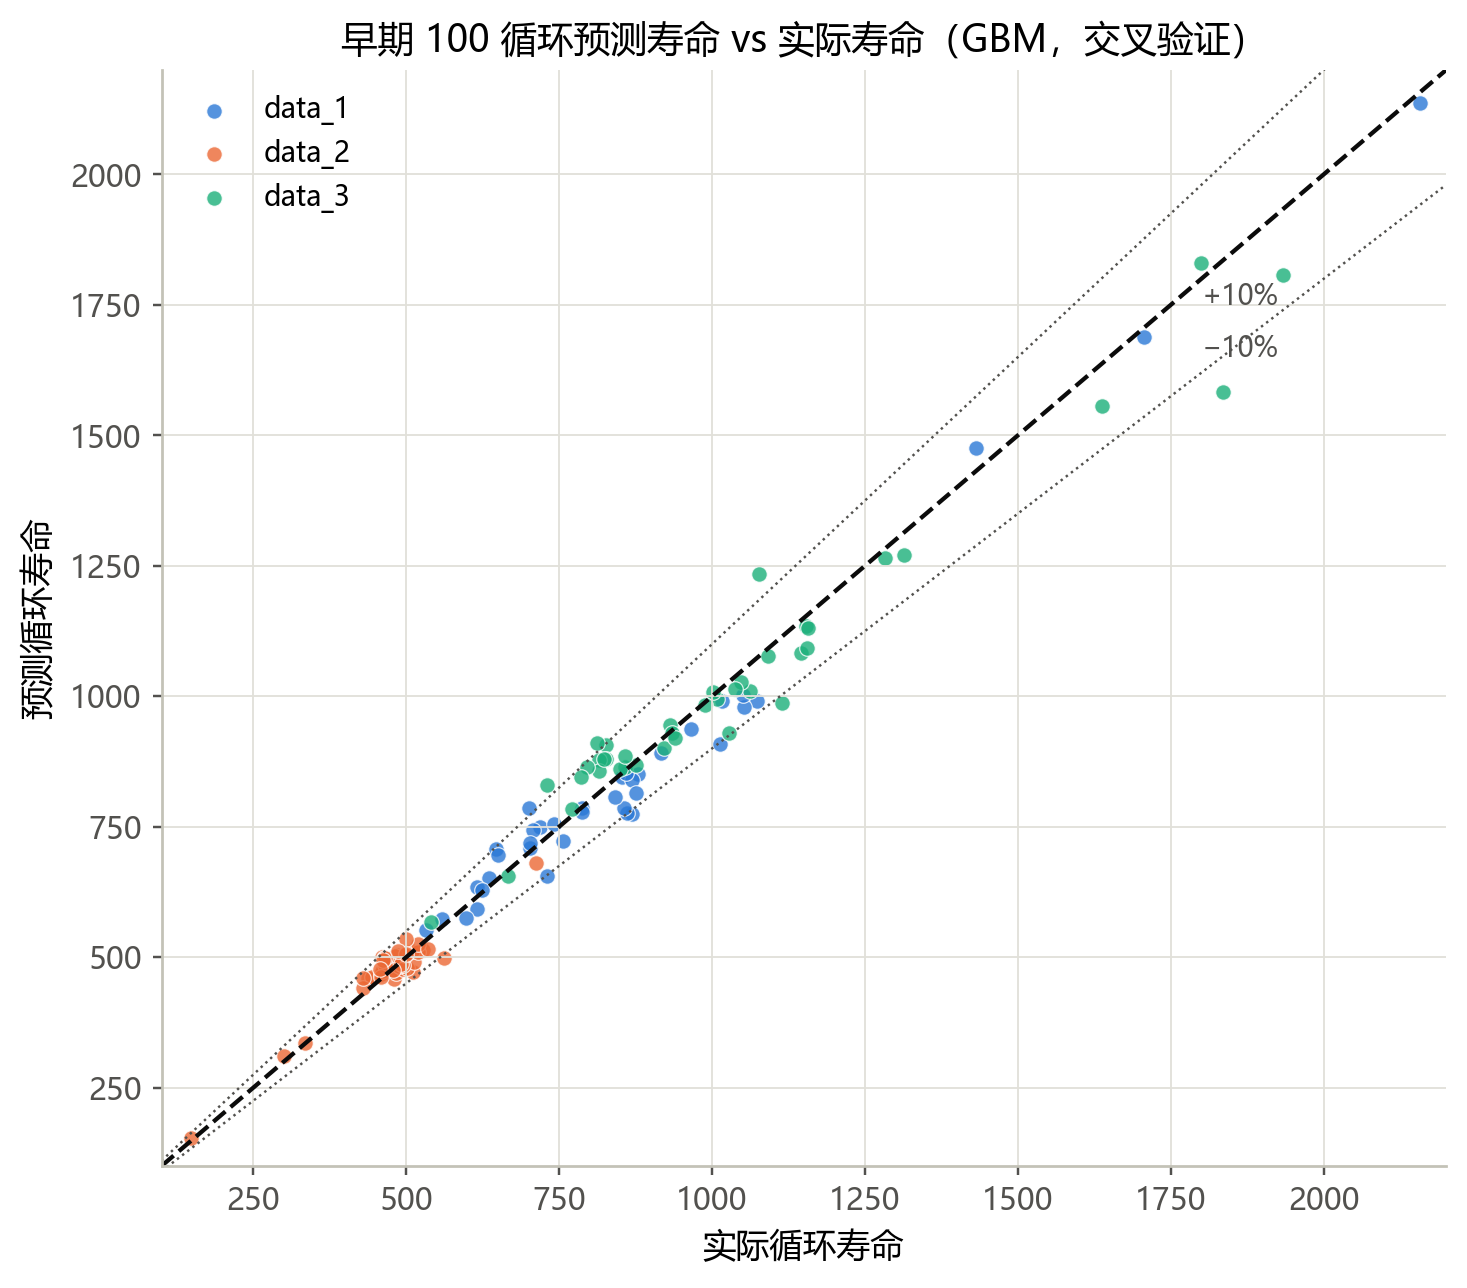
\includegraphics[width=0.75\textwidth]{figures/fig6.png}
\caption{早期 100 循环预测寿命 vs 实际寿命（GBM，交叉验证）}
\label{fig:fig6}
\end{figure}

进一步考察 $k=100$ 时 GBM 模型的预测误差分布（图 \ref{fig:fig14}）。相对误差中位数为 $+0.5\%$，90\% 的电池预测误差落在 $-11\%\sim+11\%$ 区间，误差分布对称且无系统偏差。这说明模型预测在总体上是无偏的，主要误差来源是电池个体间的不可观测差异（如初始一致性、局部工艺波动），而非特征信息的缺失。

\begin{figure}[htbp]
\centering
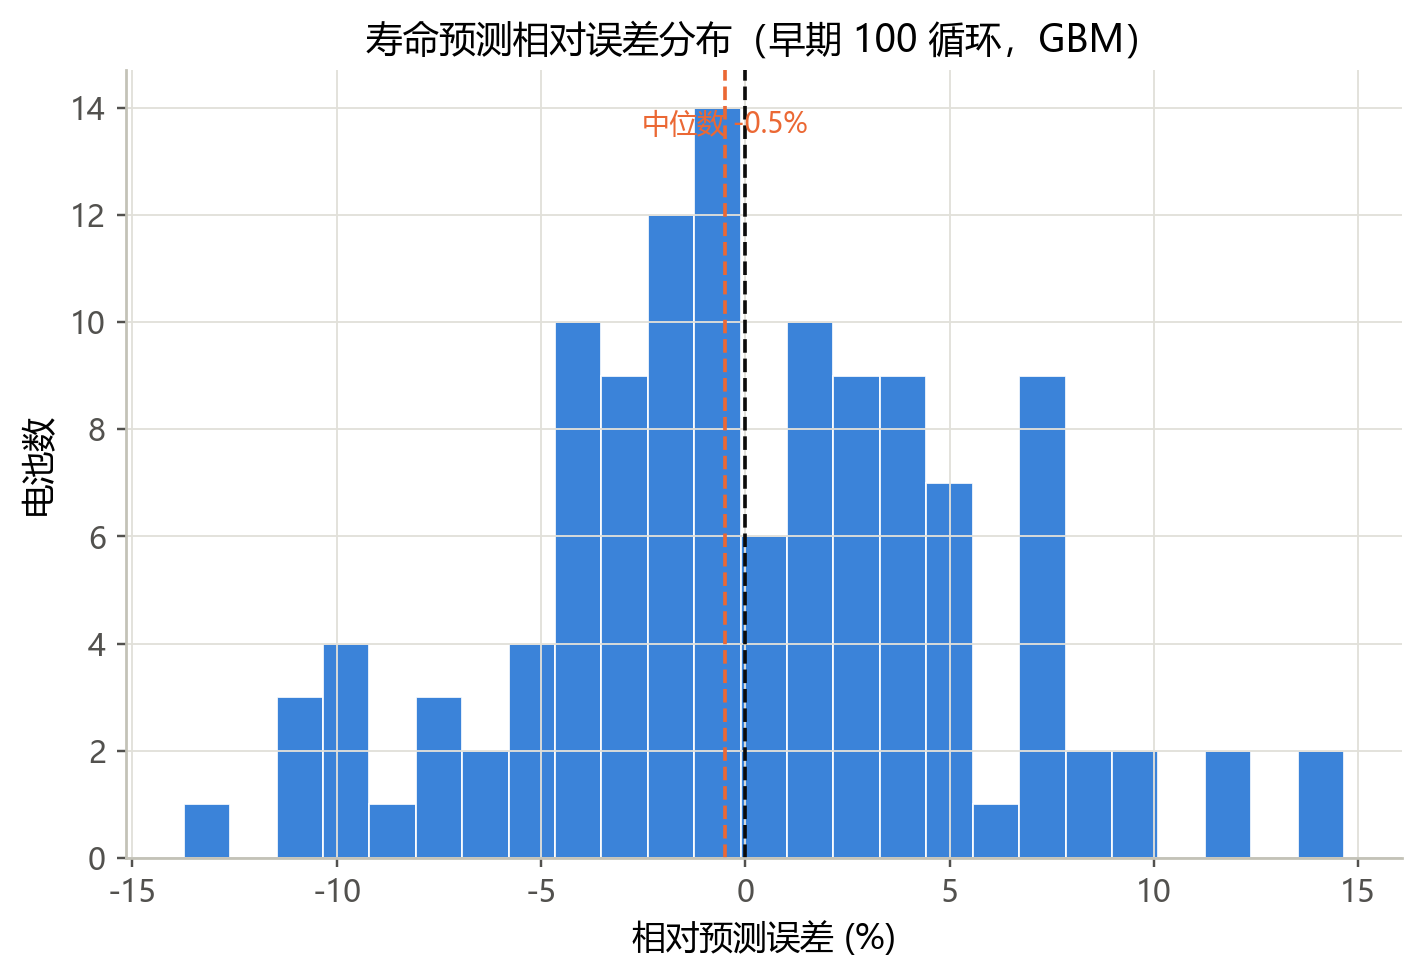
\includegraphics[width=0.62\textwidth]{figures/fig14.png}
\caption{寿命预测相对误差分布（早期 100 循环，GBM）}
\label{fig:fig14}
\end{figure}

\subsection{特征重要性分析与消融实验}

特征组合消融（表 \ref{tab:ablation}，$k=100$）：仅早期衰减特征 MAPE=16.7\%，仅策略参数 MAPE=19.7\%，二者联合 MAPE=15.0\%。早期衰减特征携带主要预测信息，策略参数提供补充。

\begin{table}[htbp]
\centering
\caption{特征组合消融（$k=100$，GBM）}
\label{tab:ablation}
\begin{tabular}{ccc}
\toprule
特征组合 & MAPE(\%) & $R^2$ \\
\midrule
仅早期衰减特征 & 16.7 & 0.735 \\
仅策略参数 & 19.7 & 0.643 \\
早期特征 + 策略参数 & 15.0 & 0.775 \\
\bottomrule
\end{tabular}
\end{table}

GBM 特征重要性（图 \ref{fig:fig8}）显示，充电时间波动（0.26）、首循环充电时间（0.19）与 SOH 残差波动（0.12）为主导特征，均刻画早期衰减信号，与利用早期容量波动预测寿命的经典思路一致。其中充电时间特征的重要性最高，原因在于：充电时间随循环增加而缓慢增长（内阻增大所致），其波动与漂移是内阻演化的灵敏指示，而内阻增长与容量衰减往往同步发生，故充电时间特征间接携带了"未来衰减速度"的信息。这一发现说明，仅依赖容量/SOH 序列或仅依赖策略参数都不足以充分利用数据，将两者联合才能获得最优预测。

\begin{figure}[htbp]
\centering
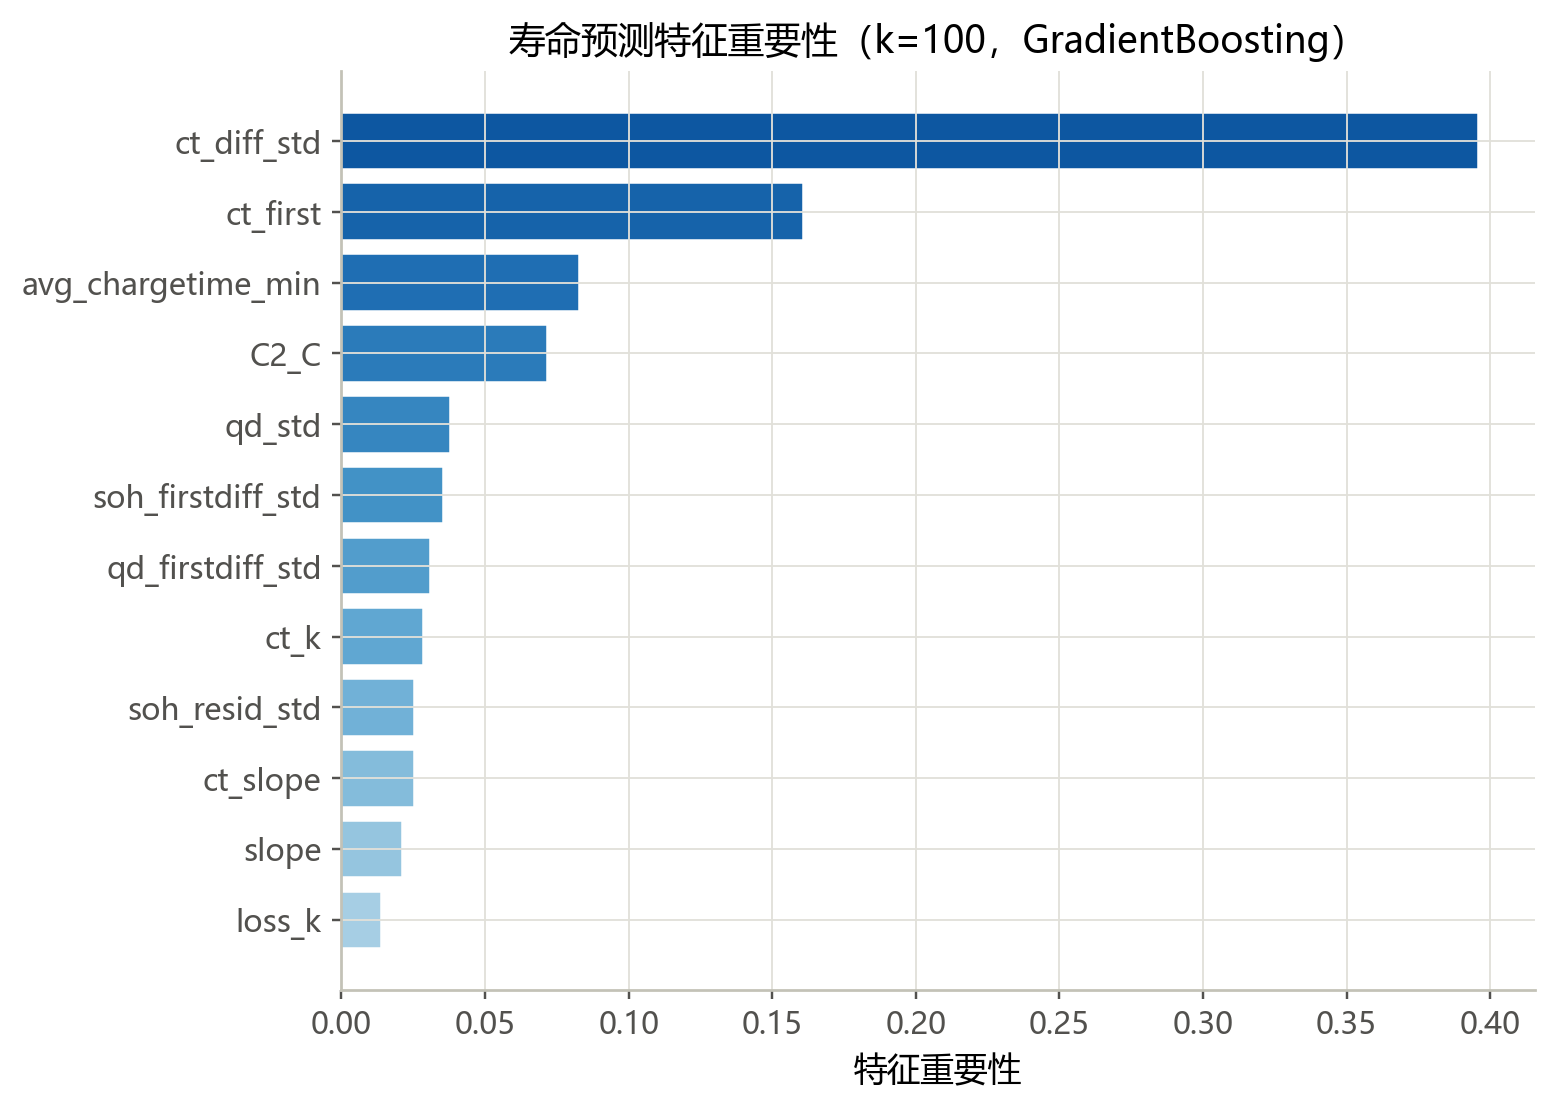
\includegraphics[width=0.75\textwidth]{figures/fig8.png}
\caption{寿命预测特征重要性（$k=100$，GBM）}
\label{fig:fig8}
\end{figure}

\subsection{未来 SOH 轨迹预测}

以 $k=20$ 特征预测里程碑循环（$t=200/400/600/800/1000$）的 SOH（表 \ref{tab:traj}）。近中期预测准确（$t\le400$ 时 MAE$\le1.2\%$），长期预测误差增大（$t\ge800$ 时 $R^2\approx0.3$、MAE 约 3\%），表明早期数据能可靠刻画近期衰减趋势，而长期 SOH 存在不可约不确定性。实际部署时可用早期数据给出寿命点估计，并随数据积累滚动更新。

\begin{table}[htbp]
\centering
\caption{里程碑 SOH 预测精度（$k=20$ 特征）}
\label{tab:traj}
\begin{tabular}{cccc}
\toprule
里程碑循环 $t$ & $R^2$ & MAE(SOH\%) & 样本数 \\
\midrule
200 & 0.628 & 0.43 & 123 \\
400 & 0.708 & 1.20 & 121 \\
600 & 0.449 & 1.98 & 80 \\
800 & 0.321 & 2.88 & 55 \\
1000 & 0.259 & 3.57 & 29 \\
\bottomrule
\end{tabular}
\end{table}

\begin{figure}[htbp]
\centering
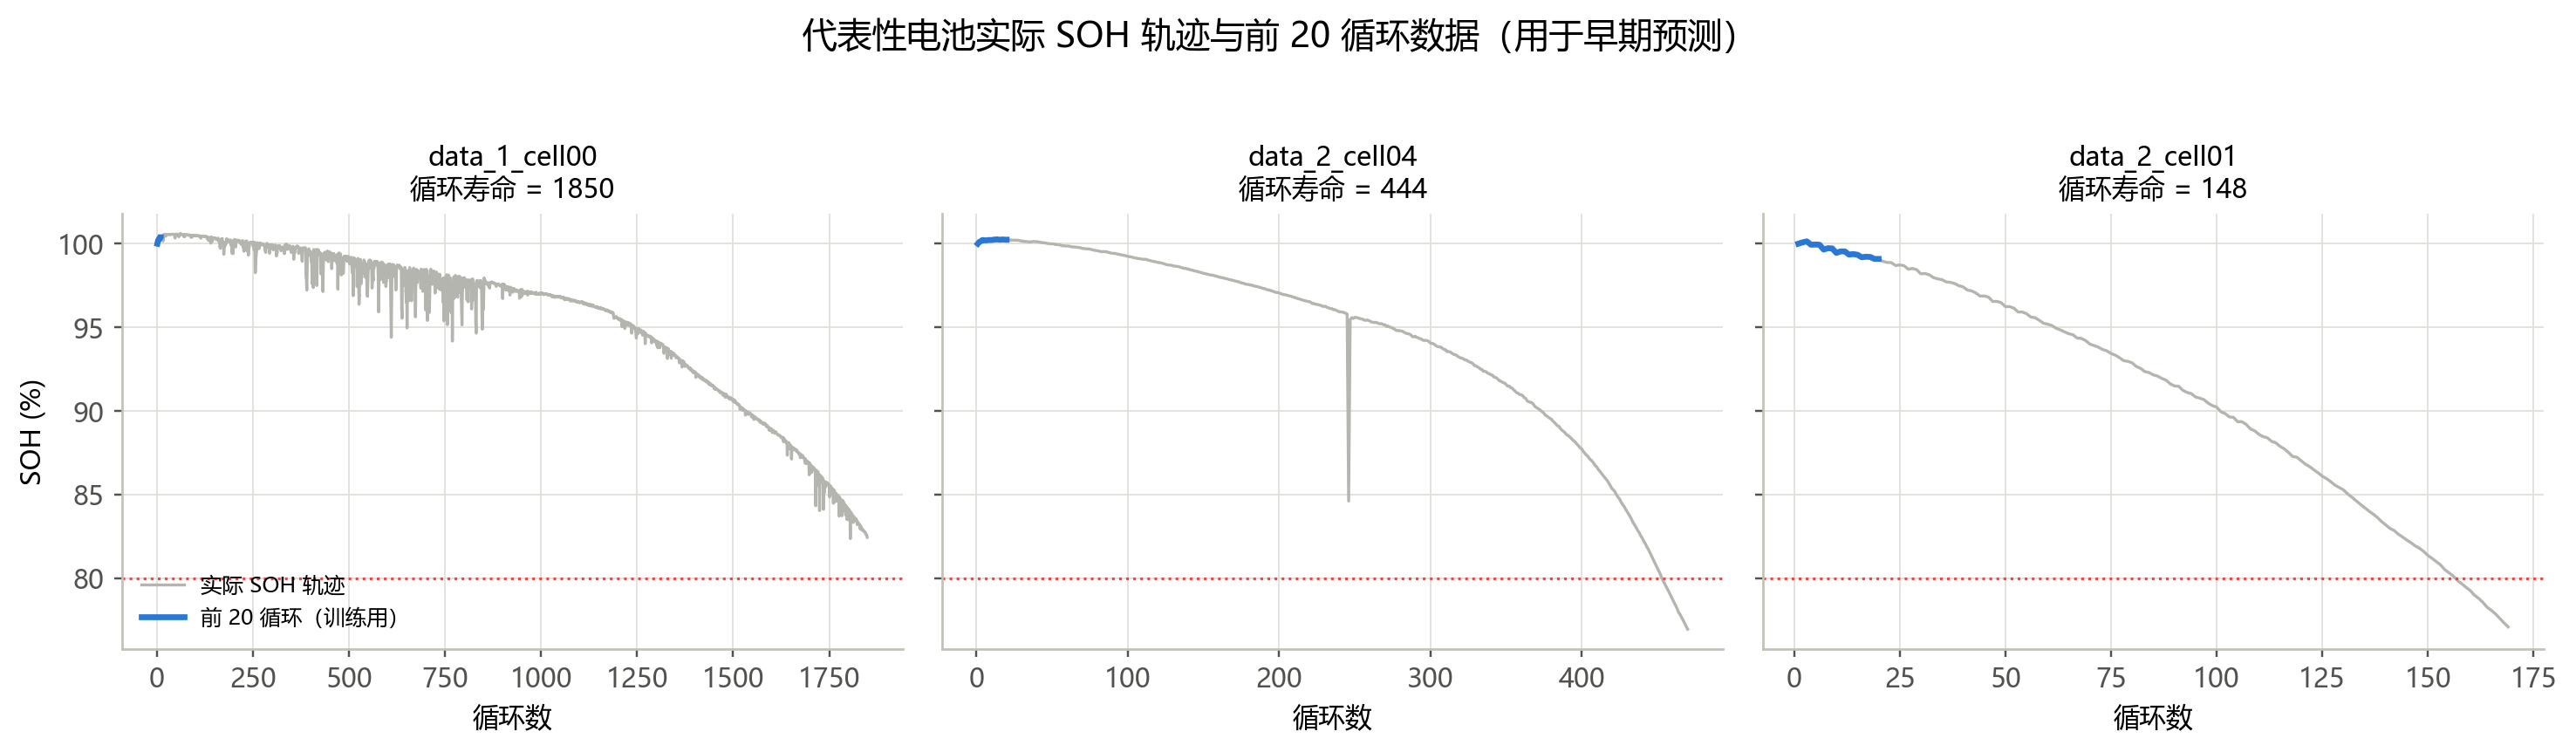
\includegraphics[width=0.95\textwidth]{figures/fig9.png}
\caption{代表性电池实际 SOH 轨迹与前 20 循环数据}
\label{fig:fig9}
\end{figure}

\subsection{充电时间漂移与内阻增长}

第 8.4 节的特征重要性分析显示充电时间特征最为关键，其机理可由图 \ref{fig:fig22} 直观说明：充电时间随循环缓慢单调上升，这是电池内阻增长导致充电效率下降的直接体现。短寿命电池的充电时间上升斜率更陡，反映其内阻增长更快；而长寿电池的充电时间几乎平稳。由于内阻增长与容量衰减源于相同的老化机制（SEI 膜增厚、活性物质损失等），充电时间的早期漂移便成为寿命的灵敏"代理信号"。这解释了为何充电时间波动/漂移特征在预测模型中的重要性最高。

\begin{figure}[htbp]
\centering
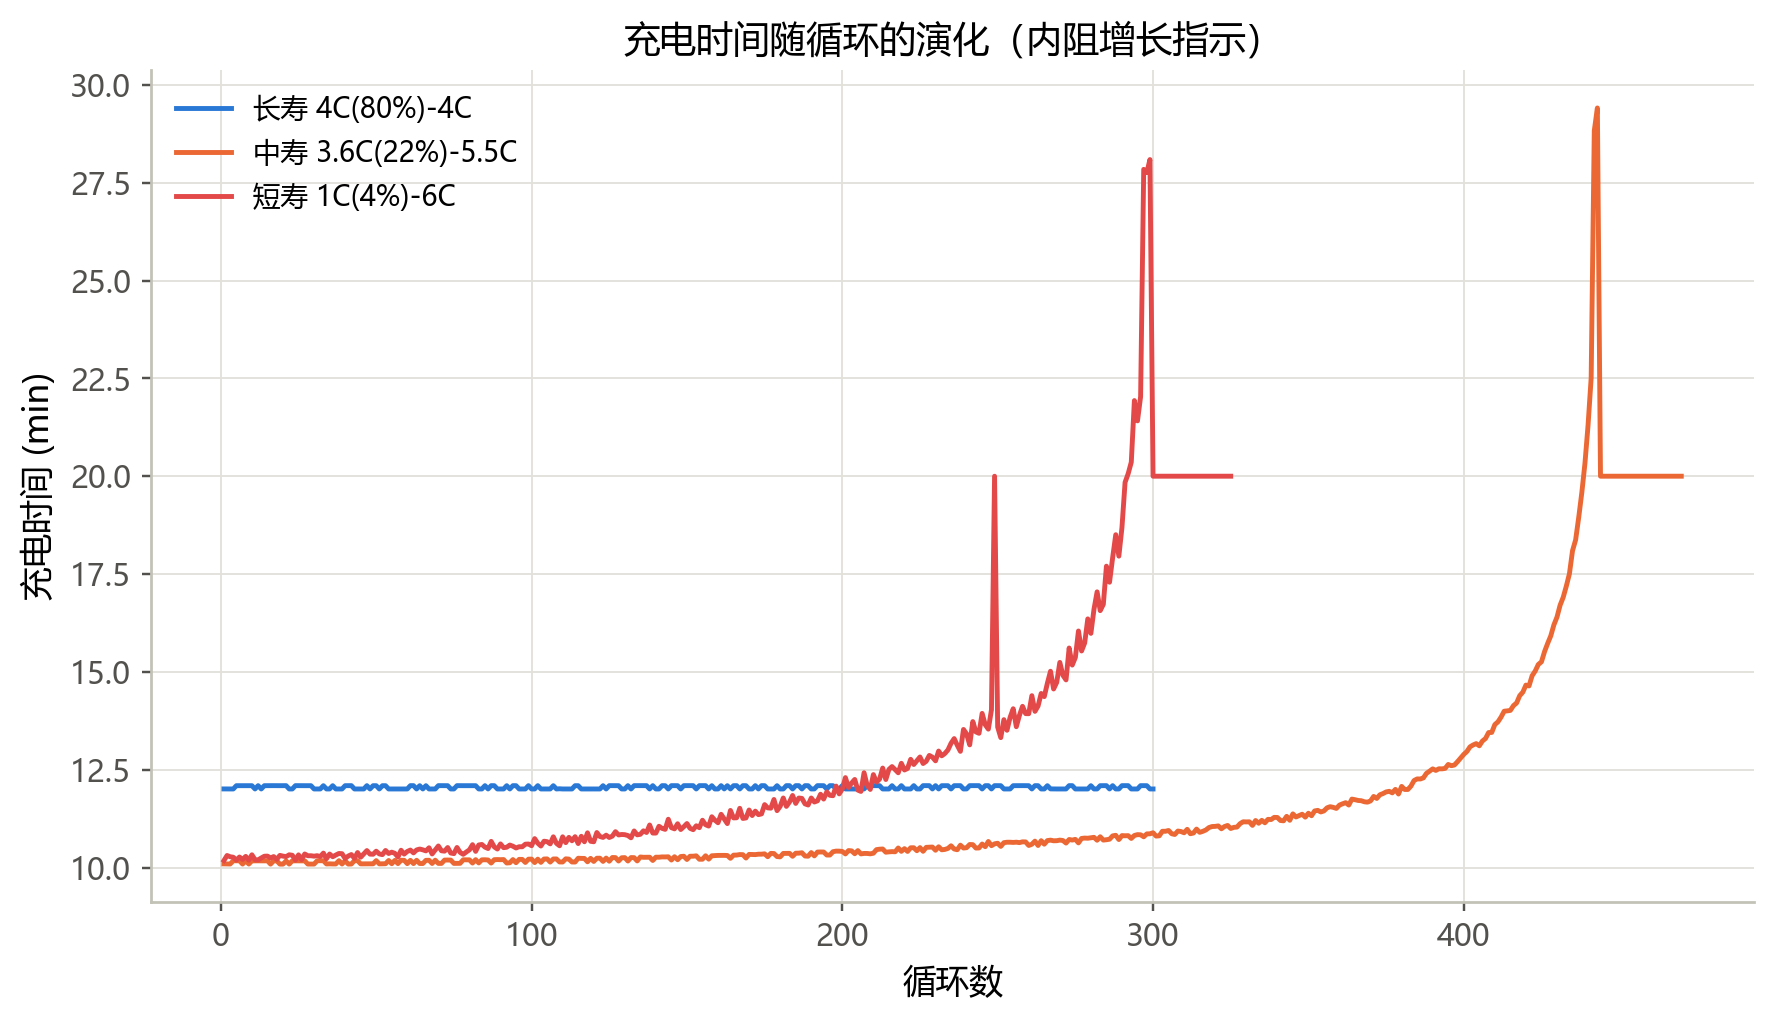
\includegraphics[width=0.72\textwidth]{figures/fig22.png}
\caption{充电时间随循环的演化（内阻增长指示）}
\label{fig:fig22}
\end{figure}

% ==================== 九、问题四 ====================
\section{问题四：兼顾充电时间与寿命衰减的策略优化模型}

\subsection{充电时间模型}

充电时间为快充段（0$\sim$80\% SOC）耗时。理想物理模型为
\begin{equation}\label{eq:T-ideal}
T_{80} = 60\cdot\frac{Q_1/100}{C_1} + 60\cdot\frac{(80-Q_1)/100}{C_2}\ \text{min}.
\end{equation}
实测数据显示高倍率下因电压限流导致实际耗时高于理想值，故拟合经验校准模型：
\begin{equation}\label{eq:T-cal}
T_{80} = 34.36\cdot\frac{Q_1/100}{C_1} + 34.03\cdot\frac{(80-Q_1)/100}{C_2} + 5.63,\quad R^2=0.365,\ \text{MAE}=0.49\ \text{min}.
\end{equation}
系数显著小于理想值 60，反映高倍率阶段受电压窗口限制、有效电流低于名义值；截距项刻画固定过程开销。

校准模型的验证结果见图 \ref{fig:fig13}：预测值与实测值相关系数 $r=0.60$，平均绝对误差 0.49 min。该模型可在设计阶段对不同策略的充电时间进行可靠估计，误差主要来源于高倍率阶段实际电流受电压窗口限制而产生的非线性，属于可接受的工程近似。

\begin{figure}[htbp]
\centering
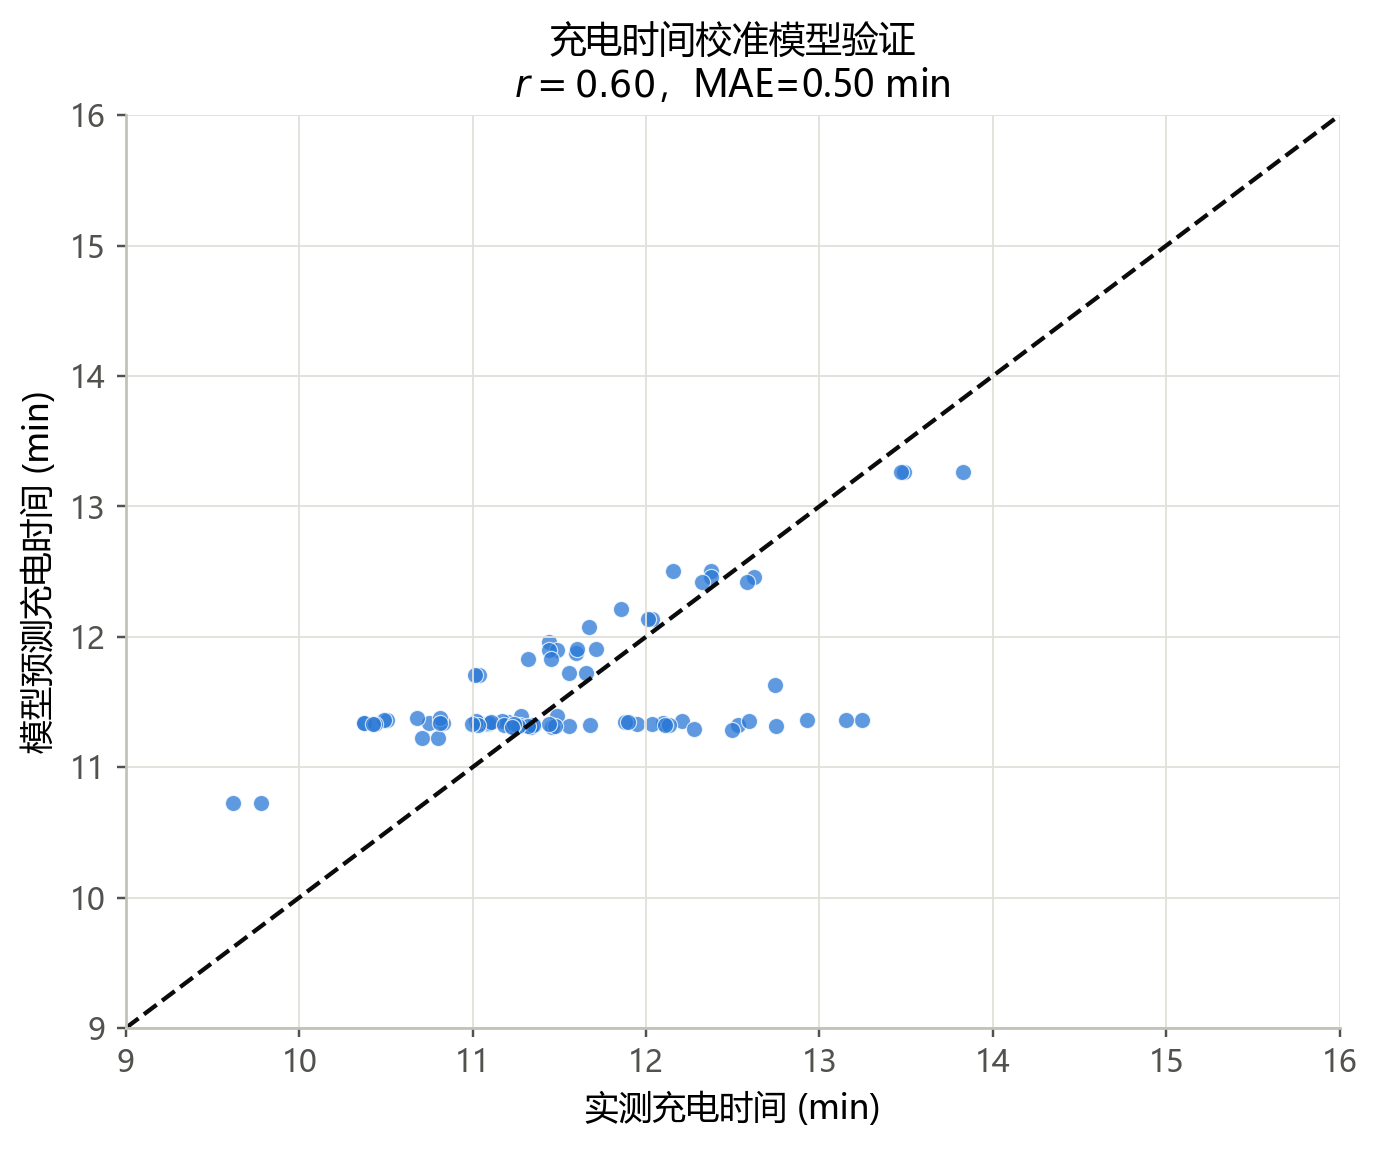
\includegraphics[width=0.6\textwidth]{figures/fig13.png}
\caption{充电时间校准模型验证（预测 vs 实测）}
\label{fig:fig13}
\end{figure}

\subsection{寿命--策略响应面}

对于尚无实测数据的候选策略，采用第 \ref{sec:dose} 节的剂量寿命模型作为设计级寿命预测；该模型与问题三的早期循环预测模型形成“先验--后验”互补：设计阶段用剂量模型给出期望寿命，运行阶段一旦积累早期循环数据，即可用问题三模型滚动更新寿命估计。设计级寿命预测模型为
\begin{equation}\label{eq:life-surface}
\log_{10}(L) = 4.312 - 0.367\,m_1 - 0.424\,m_2.
\end{equation}

\subsection{多目标优化与 Pareto 前沿}

决策变量为 $(C_1,Q_1,C_2)$，目标为最小化 $T_{80}$ 与最大化预测寿命。在观测参数水平（$C_1\in\{1,2,3.6,\ldots,8\}$，$Q_1\in\{2,\ldots,80\}$，$C_2\in\{3,\ldots,6\}$）构成的 6860 个候选组合上进行网格寻优，并以“剂量落在实测覆盖范围”（$m_1\in[0.04,4.32]$，$m_2\in[0,4.56]$）约束排除 8C(80\%) 等未经验证的极端设计，得到 6581 个可行方案与 343 个 Pareto 非支配点（图 \ref{fig:fig10}）。

\begin{figure}[htbp]
\centering
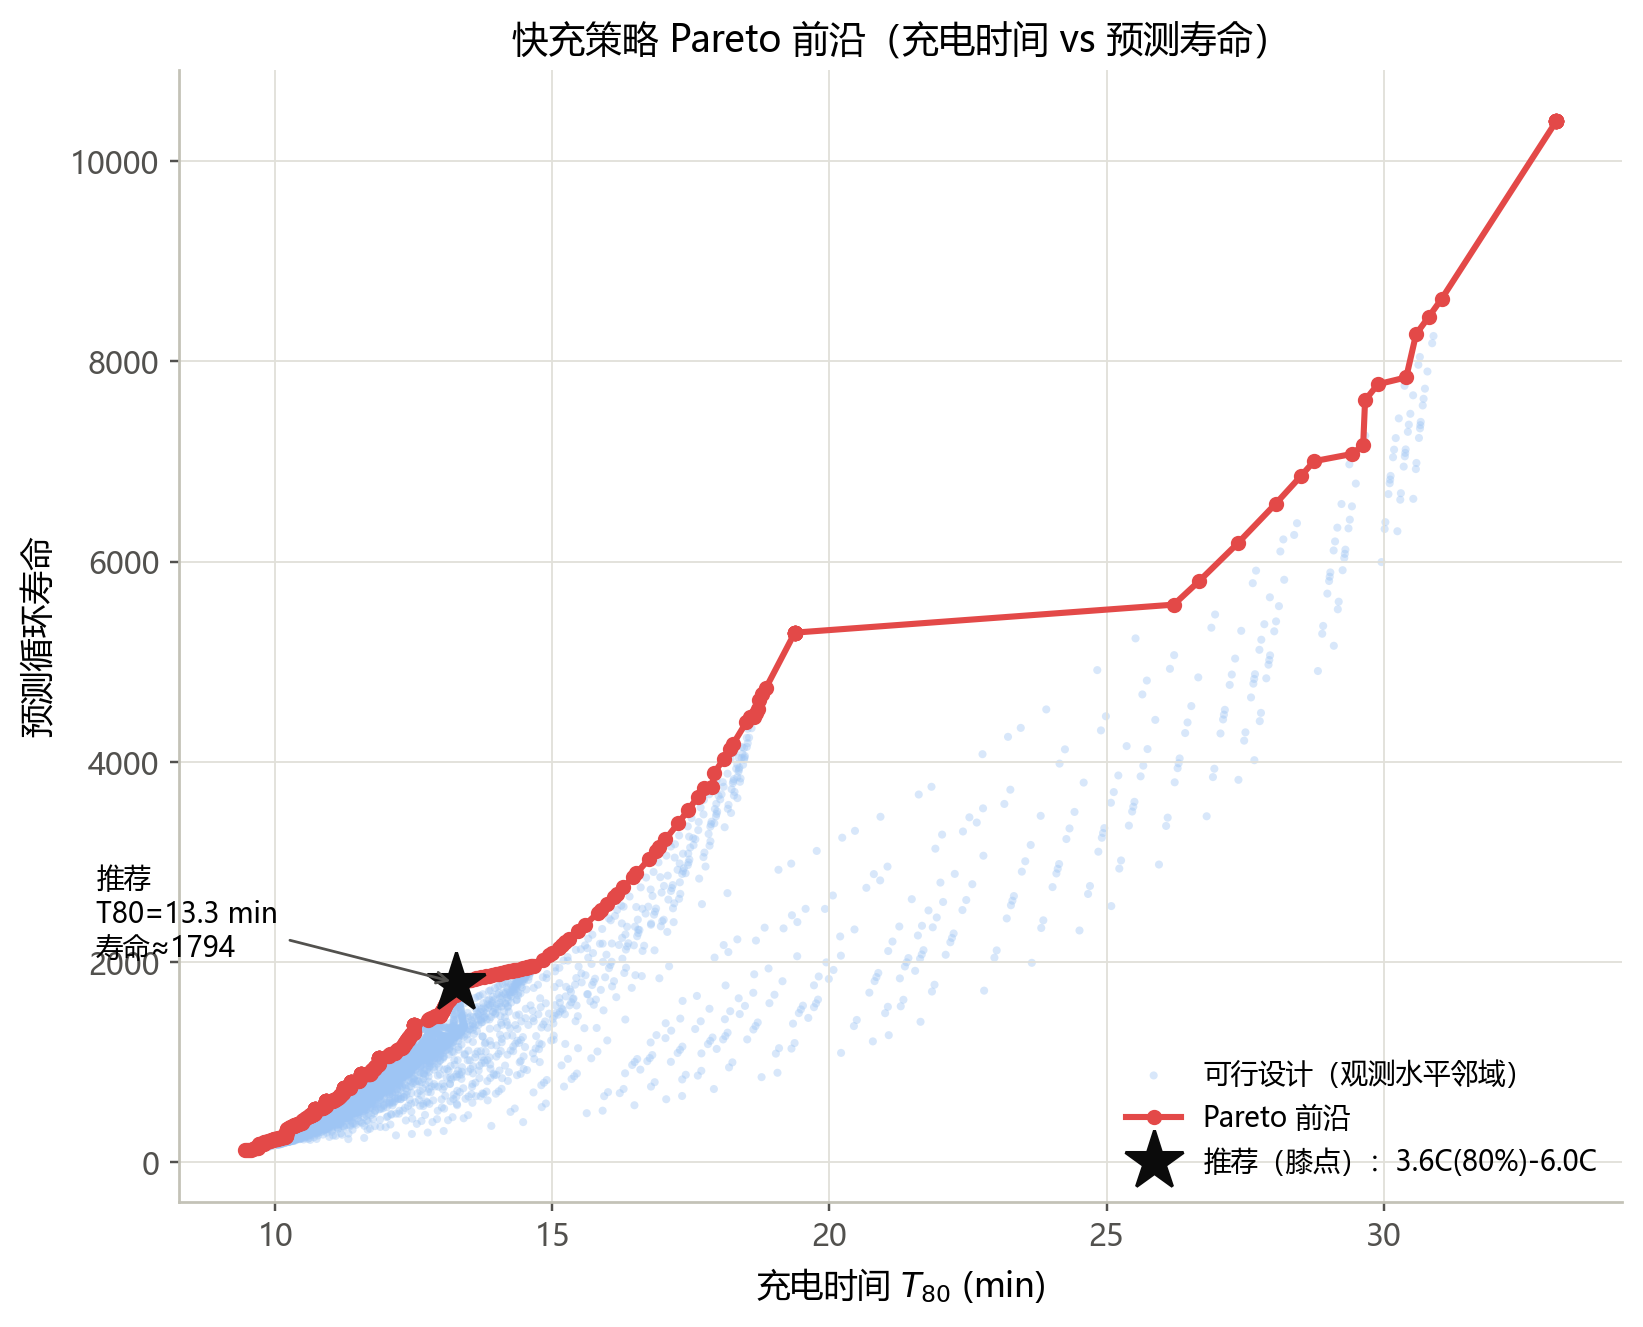
\includegraphics[width=0.8\textwidth]{figures/fig10.png}
\caption{快充策略 Pareto 前沿（充电时间 vs 预测寿命）}
\label{fig:fig10}
\end{figure}

Pareto 前沿清晰呈现“充电时间越短、预测寿命越短”的权衡（图 \ref{fig:fig10}）。前沿的左端为快而短命的激进攻略（$T_{80}\approx9.3$ min、寿命约 280），右端为慢而长寿的温和策略（$T_{80}\approx35$ min、寿命约 2320），中间为连续权衡带。由于寿命在 $\log$ 尺度上随充电时间近似呈"S 形"增长，存在一个边际收益骤降的拐点区域，即"膝点"：在该点之前，增加少量充电时间即可换取大幅寿命提升；在该点之后，继续增加充电时间收益甚微。

采用归一化对数寿命空间中"离端点连线最远的点"作为膝点推荐，得到策略 3.6C(80\%)-3.6C，其恰好落在数据已验证的长寿策略区域，形成模型与实验的互相印证。这一膝点选择既避免了过度追求寿命（充电时间过长、失去快充意义），也避免了过度压缩时间（寿命过短、得不偿失），是在"快充"与"长寿"之间的平衡选择。

\subsection{推荐策略与对比}

推荐策略 3.6C(80\%)-3.6C：先以 3.6C 充电至 80\% SOC，再 1C CC-CV 至满电。预测充电时间 13.3 min、预测寿命 1794，数据实测平均寿命 2081（批次 1，$n=3$）。更快备选 4C(80\%)-4C：充电时间 12.5 min、预测寿命 1369、实测寿命 1570（$n=2$）。两者与短寿命策略形成鲜明对比（表 \ref{tab:compare}、图 \ref{fig:fig11}）。

\begin{table}[htbp]
\centering
\caption{推荐策略与典型策略对比}
\label{tab:compare}
\begin{tabular}{ccccccc}
\toprule
策略 & $C_1$(C) & $Q_1$(\%) & $C_2$(C) & $T_{80}$(min) & 预测寿命 & 实测寿命 \\
\midrule
\textbf{推荐 3.6C(80\%)-3.6C} & 3.6 & 80 & 3.6 & 13.3 & 1794 & \textbf{2081} \\
\textbf{备选 4C(80\%)-4C} & 4.0 & 80 & 4.0 & 12.5 & 1369 & \textbf{1570} \\
8C(15\%)-3.6C & 8.0 & 15 & 3.6 & 12.4 & 756 & 1008 \\
6C(30\%)-3.6C & 6.0 & 30 & 3.6 & 12.1 & 772 & 1013 \\
1C(4\%)-6C & 1.0 & 4 & 6.0 & 11.3 & 231 & 300 \\
2C(10\%)-6C & 2.0 & 10 & 6.0 & 11.3 & 287 & 148 \\
\bottomrule
\end{tabular}
\end{table}

\begin{figure}[htbp]
\centering
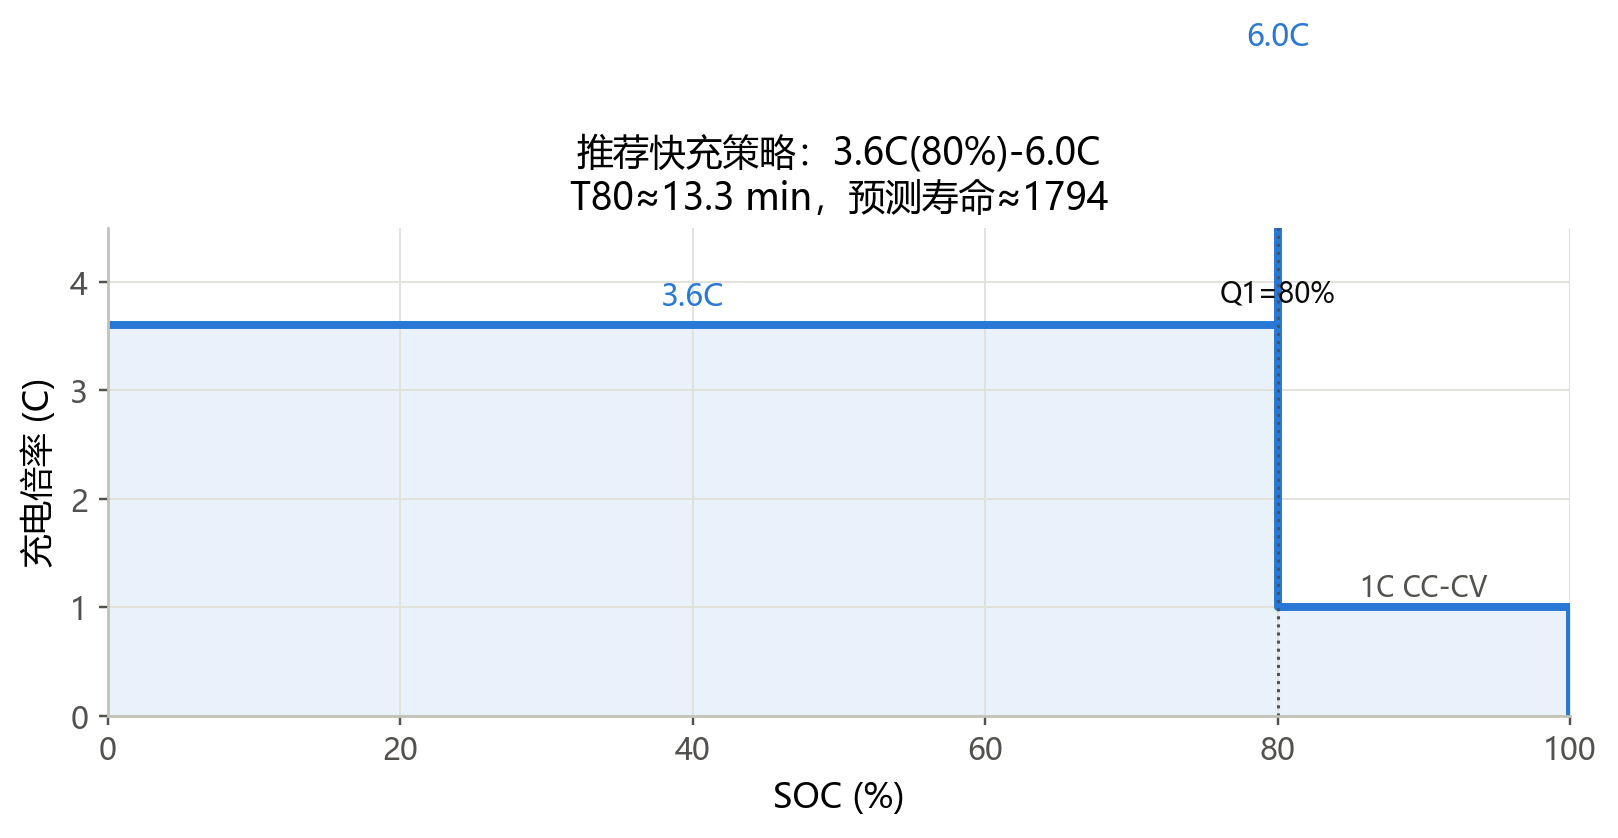
\includegraphics[width=0.8\textwidth]{figures/fig11.png}
\caption{推荐快充策略电流剖面（3.6C(80\%)-3.6C）}
\label{fig:fig11}
\end{figure}

图 \ref{fig:fig15} 直观对比了推荐策略、备选策略与典型长/短寿命策略的实测寿命与充电时间。推荐策略 3.6C(80\%)-3.6C 在充电时间几乎不增加的前提下，实测寿命比短寿命策略（1C(4\%)-6C 的 300、2C(10\%)-6C 的 148）高出 4$\sim$8 倍，体现了“不牺牲充电时间的前提下显著延长寿命”的优化效果；备选策略 4C(80\%)-4C 进一步将充电时间压缩至 12.5 min，寿命仍高达 1570。

\begin{figure}[htbp]
\centering
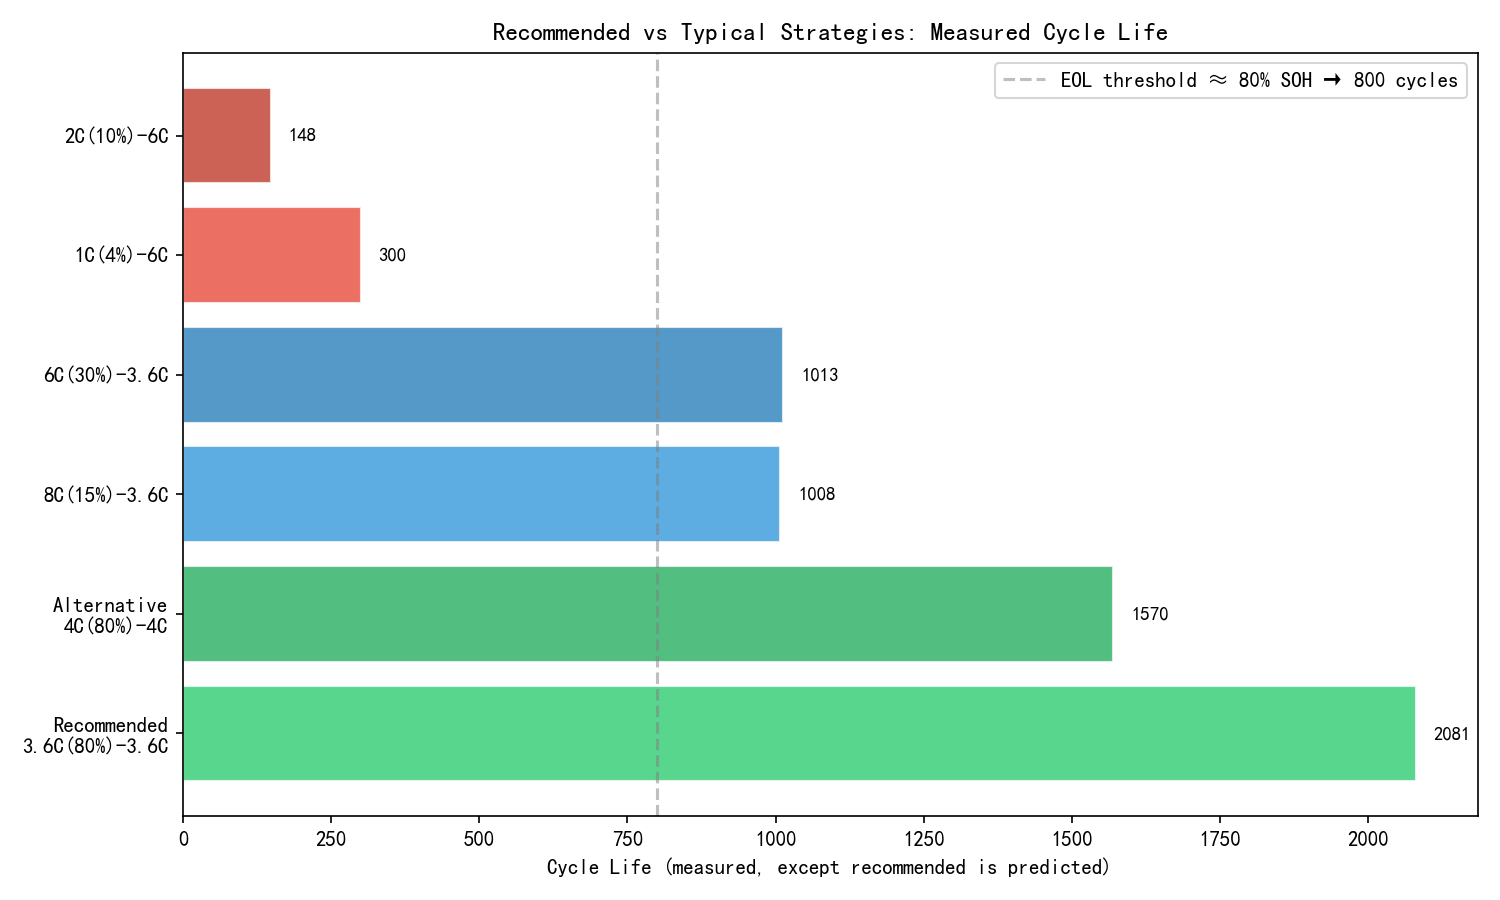
\includegraphics[width=0.92\textwidth]{figures/fig15.png}
\caption{推荐策略与典型策略的实测寿命与充电时间对比}
\label{fig:fig15}
\end{figure}

\subsection{合理性、适用范围与外推风险}

（1）\textbf{合理性}：推荐策略以“中高 SOC 区间低倍率充电”为核心机理（$m_2\approx0$），在几乎不延长充电时间（13.3 min）的前提下实现长寿，与问题二结论一致；优化器收敛到实验已验证的长寿策略，佐证了模型与方法的可信度。

（2）\textbf{适用范围}：模型基于 A123 18650 LFP 电池在给定实验协议下的数据，适用于同类型电池、0$\sim$80\% 快充段、常温条件；批次间存在系统性差异，绝对寿命预测应按目标批次重新标定。

（3）\textbf{外推风险}：优化结果被严格限制在实测参数水平及其剂量覆盖范围之内，未对未经验证的高倍率--高 SOC 组合（如 8C 充至 80\%）外推；若扩展至高倍率或更宽 SOC 区间，应补充实验数据并重新拟合，避免线性模型在支持域外失效。

（4）\textbf{工程实现考虑}：推荐策略为两段式恒流充电（3.6C 至 80\% SOC 后 1C CC-CV），工程上易于在现有充电机与电池管理系统（BMS）中实现——只需将 BMS 的充电电流-电压曲线按该方案配置即可。实际落地时还应注意：低温下 3.6C 充电可能导致负极析锂风险上升，需结合温度约束动态降额；CC-CV 阶段的 80\%$\sim$100\% 补电时间受电化学极化影响，应在总补能时间估算中一并计入。这些工程细节不改变本文的定性结论，但影响具体的参数标定。

% ==================== 十、模型的检验与灵敏度分析 ====================
\section{模型的检验与灵敏度分析}

\subsection{寿命模型交叉验证}

采用 5 折交叉验证检验剂量寿命模型的预测稳定性：在全部 standard 数据上 $R^2=0.608$；而单独在批次 1 内交叉验证，$R^2=0.848$。两者差异说明模型在批次内解释力强、预测稳定，跨批次合并数据则稀释了预测精度，进一步印证了批次效应的存在。

\subsection{留一批次外推检验}

为定量刻画批次效应，做留一批次外推检验：用批次 1 训练、批次 2 检验，寿命 MAPE 达 64\%（$R^2<0$）；反向亦为 38\%（$R^2<0$）。这说明\textbf{绝对寿命的跨批次外推不可靠}，模型捕获的是批次内的相对关系，与第 5 节“批次效应说明”及第 9 节“绝对寿命预测应按目标批次重新标定”的结论一致。因此，本文推荐策略的价值在于给出批次内的最优相对设计，而非跨批次的绝对寿命保证；实际部署时需结合目标批次数据重新标定后再做绝对寿命判断。

\subsection{推荐策略灵敏度分析}

对推荐策略 3.6C(80\%)-3.6C 的三个参数分别施加扰动，考察充电时间与预测寿命的变化（表 \ref{tab:sens}）：
\begin{itemize}
\item \textbf{$C_1$ 是主要敏感参数}：$C_1$ 每变化 $\pm0.4$C，充电时间反向变化约 6\%$\sim$8\%，预测寿命反向变化约 12\%$\sim$13\%，二者权衡明显——$C_1$ 提高可加速充电但明显缩短寿命。实际执行中应重点保证 $C_1$ 的准确性。
\item \textbf{$Q_1$、$C_2$ 扰动影响可忽略}：因 $Q_1=80\%$ 时第二阶段覆盖为零、$C_2$ 不参与快充段充电，故 $C_2$ 的扰动不影响结果，$Q_1$ 略降影响也甚微。这提示推荐策略对 $C_2$、$Q_1$ 的小幅执行偏差具有鲁棒性。
\end{itemize}

\begin{table}[htbp]
\centering
\caption{推荐策略参数灵敏度分析（基准 3.6C(80\%)-3.6C）}
\label{tab:sens}
\begin{tabular}{llcc}
\toprule
参数扰动 & 变化 & $T_{80}$(min) & 预测寿命 \\
\midrule
基准 & --- & 13.3 & 1794 \\
$C_1$ & $+0.4$C & 12.5（$-5.8\%$） & 1369（$-23.7\%$） \\
$C_1$ & $-0.4$C & 14.2（$+7.2\%$） & 2351（$+31.1\%$） \\
$Q_1$ & $-5\%$ & 13.3（$0\%$） & 1752（$-2.3\%$） \\
$C_2$ & $\pm0.4$C & 13.3（$0\%$） & 1794（$0\%$） \\
\bottomrule
\end{tabular}
\end{table}

% ==================== 十一、模型评价、改进与推广 ====================
\section{模型评价、改进与推广}

\subsection{模型优点}
\begin{enumerate}
\item \textbf{机理与数据结合}：剂量模型以“高倍率电量在 SOC 轴上的分布”刻画老化，系数符号与电化学机制一致，结果可解释。
\item \textbf{充分考虑混杂与批次效应}：多变量回归引入批次虚拟变量，分批次回归作为稳健性验证，结论不依赖于单一批次。
\item \textbf{预测模型经严格交叉验证}：5 折$\times$8 次重复交叉验证避免过拟合，并给出不同早期窗口的精度-成本权衡。
\item \textbf{优化约束合理}：设计空间严格限制在实验覆盖范围，避免过度外推。
\end{enumerate}

\subsection{模型不足与改进}
\begin{enumerate}
\item 问题二回归模型仅解释约 62\%（含批次）的寿命方差，电池个体差异与温度等未观测因素仍占较大比例；可引入温度、内阻等逐循环协变量提高解释力。
\item 问题三长期 SOH 预测精度较低（$t\ge800$ 时 $R^2\approx0.1$），可结合电化学模型或序列模型（LSTM/Transformer）刻画长期非线性衰减。
\item 问题四以充电倍率与 SOC 切换点为决策变量，未考虑电流阶跃、温度约束等工程细节，实际落地需结合热管理进行仿真验证。
\end{enumerate}

\subsection{模型推广}
本模型框架可推广至其他电池体系（如三元锂电池、钠离子电池）及其他充电协议（脉冲充电、多段电流），只需重新拟合剂量-寿命响应面与早期预测特征即可；“先验（策略剂量）--后验（早期数据）”结合的策略优化范式具有通用性。

\subsection{建模方法总结}

本文形成了一套面向快充策略设计的"整理--量化--预测--优化"闭环方法：首先通过数据整理将原始循环时序压缩为可建模的策略参数与寿命标签；其次用"剂量"视角将充电策略投影到 SOC 轴上的高倍率电量分布，建立机理可解释的寿命响应面；再次以早期衰减特征为代理，实现无需长期试验的寿命快速预测；最后在实验覆盖的合理邻域内以 Pareto 前沿给出兼顾充电时间与寿命的设计方案。该方法的核心价值在于将"电化学机理认知"转化为"可计算的剂量-响应关系"，使快充策略设计从经验试错走向定量寻优。

% ==================== 十二、结论 ====================
\section{结论}

本文围绕快充策略对锂离子电池寿命衰减的影响，完成了“数据整理 $\rightarrow$ 量化建模 $\rightarrow$ 寿命预测 $\rightarrow$ 策略优化”四个递进环节，主要结论如下：

\begin{enumerate}
\item \textbf{数据与寿命分布}：完成 124 个电池策略参数、寿命、SOH 曲线与充电时间的系统整理；寿命跨度约 15 倍（148$\sim$2235），策略影响极显著；三个批次寿命中位数分别为 841、481、964。
\item \textbf{量化模型}：$C_2$ 是主要的负向倍率策略因素（含批次标准化系数 $-0.040$，偏相关 $-0.250$），充电时间 $T_{80}$ 与寿命正相关（偏相关 $+0.363$）；单位高倍率电量在中高 SOC 区间的寿命损伤比低 SOC 区间高约 16\%（$m_2$ $-0.424$ vs $m_1$ $-0.367$），验证了不同 SOC 区间高倍率影响的显著差异；$C_1\times Q_1$、$C_2\times Q_1$ 交互项从剂量角度解释了各参数的作用机制。
\item \textbf{寿命预测}：基于早期 20 个循环特征（SOH 衰减率、波动、充电时间漂移），GBM 模型交叉验证 MAPE=15.3\%、$R^2=0.77$；充电时间波动与 SOH 残差波动为主导特征；近中期 SOH 预测误差小于 1.2\%，长期 SOH 存在不可约不确定性。
\item \textbf{策略优化}：在实验覆盖邻域内得到 Pareto 前沿，推荐 3.6C(80\%)-3.6C（充电 13.3 min、实测寿命 2081）与更快备选 4C(80\%)-4C（12.5 min、实测 1570），实现“不牺牲充电时间的快速补能与显著寿命延长”；结果限定在数据覆盖范围内，并给出外推风险边界。
\end{enumerate}

\textbf{展望。}本文采用的"剂量--响应--预测--优化"框架尚有进一步拓展空间：其一，将逐循环温度、内阻等协变量纳入剂量模型，有望解释残余的电池个体差异，进一步提高 $R^2$；其二，引入循环衰减的电化学机理模型（如固体电解质界面膜生长模型）与机器学习结合，可提升长期 SOH 预测的外推能力；其三，将优化从"两段式策略"推广到任意 SOC 分段的电流曲线设计，并叠加温度与电压约束，可得到更贴近工程实际的充电方案。这些方向将在后续工作中探索。

% ==================== 参考文献 ====================
\begin{thebibliography}{9}
\bibitem{ref1} Severson K A, Attia P M, Jin N, et al. Data-driven prediction of battery cycle life before capacity degradation[J]. Nature Energy, 2019, 4(5): 383-391.
\end{thebibliography}

% ==================== 附录 ====================
\begin{appendices}

\section{支撑材料文件列表}

本论文的支撑材料文件列表如表 \ref{tab:support} 所示。所有源程序可运行，分析结果与本论文一致。

\begin{table}[htbp]
\centering
\caption{支撑材料文件列表}
\label{tab:support}
\begin{tabular}{lll}
\toprule
文件名 & 内容 & 用途 \\
\midrule
data\_1.mat / data\_2.mat / data\_3.mat & 三个批次原始循环老化数据 & 数据来源 \\
data\_extract.py & 从 HDF5 提取电池级汇总表 & 数据整理 \\
build124.py & 合并延续电池并筛选 124 个有效电池 & 数据整理 \\
analysis2.py & 问题二回归/剂量/交互分析 & 问题二 \\
analysis3.py & 问题三特征提取与预测 & 问题三 \\
analysis4.py & 问题四充电时间/寿命模型与优化 & 问题四 \\
battery\_table\_124.csv & 124 电池汇总表 & 中间数据 \\
每循环明细表\_124.csv & 逐循环 SOH/容量/充电时间 & 中间数据 \\
\bottomrule
\end{tabular}
\end{table}

\section{源程序}

以下为主要分析源程序（Python）。运行环境：Python 3.10+，依赖 numpy、pandas、scipy、matplotlib、scikit-learn、h5py。注意脚本中数据路径需按实际位置修改。

\subsection{data\_extract.py —— 数据提取}
\lstinputlisting[language=Python]{code/data_extract.py}

\subsection{build124.py —— 数据筛选（合并延续电池、构建 124 电池集）}
\lstinputlisting[language=Python]{code/build124.py}

\subsection{analysis1.py —— 问题一：数据整理与初步分析}
\lstinputlisting[language=Python]{code/analysis1.py}

\subsection{analysis2.py —— 问题二：量化模型}
\lstinputlisting[language=Python]{code/analysis2.py}

\subsection{analysis3.py —— 问题三：寿命预测模型}
\lstinputlisting[language=Python]{code/analysis3.py}

\subsection{analysis4.py —— 问题四：策略优化}
\lstinputlisting[language=Python]{code/analysis4.py}

\end{appendices}

\end{document}
